%% -------------------------------------------------------------
%% ms.tex -- MAIN FILE (the one that you compile with LaTeX)
%% -------------------------------------------------------------

% Set up the document

\documentclass[a4paper, 11pt, oneside]{Thesis}  % Use the "Thesis" style, based
                                                % on the ECS Thesis style by
                                                % Steve Gunn
\graphicspath{Figures/}  % Location of the graphics files (set up for graphics
                         % to be in PDF format)

% Include any extra LaTeX packages required
\usepackage[backend=biber]{biblatex}
\addbibresource{ms.bib}

\usepackage{verbatim}   % Needed for the "comment" environment to make LaTeX
                        % comments
\usepackage{sty/vector}     % Allows "\bvec{}" and "\buvec{}" for "blackboard"
                        % style bold vectors

\hypersetup{urlcolor=blue, colorlinks=true}

\usepackage{tikz}  % for drawing graphs and diagrams
\usetikzlibrary{
  shapes.multipart,
  shapes.geometric,
  arrows,
  fit,
  matrix,
  positioning,
  shapes.callouts,
  shapes.arrows,
  calc
}

\usepackage{pgfplots}
\pgfplotsset{compat=1.10}
\usetikzlibrary{shapes.geometric,arrows,fit,matrix,positioning}

\definecolor{myyellow}{RGB}{245,177,0}
\definecolor{mysalmon}{RGB}{255,145,73}

\usepackage{amsmath}
\usepackage{mathtools}
\DeclarePairedDelimiter\ceil{\lceil}{\rceil}
\DeclarePairedDelimiter\floor{\lfloor}{\rfloor}

\usepackage[xindy,toc]{glossaries}
\newglossaryentry{processor}{
    name=processor,
    description={A device that can perform a sequence of operations, one
    operation per unit time, and can that access memory in its shared memory
    region.}
}
\newglossaryentry{p}{
    name=p,
    description={a variable referring to a processor or indicating association
    to a processor}
}

\newglossaryentry{conflict detection function}{
    name={\texttt{conflicted}, $C$},
    description={A function associated with an operation $f$ that detects if a
    value in a P/T data structure was computed using a stale value}
}

\newglossaryentry{resolution function}{
    name={\texttt{resolve}, $R$},
    description={A function associated with an operation $f$ that resolves a
    conflicted value in a P/T data structure so that it corresponds to the
    correct value of an input to $f$.}
}

























\loadglsentries[main]{Chapters/07_Glossary}
\makeglossaries

% commands
\newcommand{\Op}{\mathrm{\mathbf{Op}}}
\newcommand{\Ev}{\mathbf{E}}

%% ----------------------------------------------------------------
\begin{document}
\frontmatter      % Begin Roman style (i, ii, iii, iv...) page numbering

% Set up the Title Page
\title  {Persistent Data Models for Automatic Parallelization of Nontrivial
            Communication Patterns}
\authors  {\texorpdfstring
            {\href{your web site or email address}{Sean Laguna}}
            {Sean Laguna}
            }
% Do not change this here, instead these must be set in the "ms.cls" file,
% please look through it instead
\addresses  {\groupname\\\deptname\\\univname}
\date       {\today}
\subject    {}
\keywords   {}

\maketitle
%% ----------------------------------------------------------------

\setstretch{1.15}   % It is better to have smaller font and larger line spacing
                    % than the other way round

% Define the page headers using the FancyHdr package and set up for one-sided
% printing
\fancyhead{}        % Clears all page headers and footers
\rhead{\thepage}    % Sets the right side header to show the page number
\lhead{}            % Clears the left side page header

\pagestyle{fancy}   % Finally, use the "fancy" page style to implement the
                    % FancyHdr headers

%% ----------------------------------------------------------------
% Declaration Page required for the Thesis, your institution may give you a different text to place here
%\Declaration{
%
%\addtocontents{toc}{\vspace{1em}}  % Add a gap in the Contents, for aesthetics
%
%I, AUTHOR NAME, declare that this thesis titled, `THESIS TITLE' and the work presented in it are my own. I confirm that:
%
%\begin{itemize}
%\item[\tiny{$\blacksquare$}] This work was done wholly or mainly while in candidature for a research degree at this University.
%
%\item[\tiny{$\blacksquare$}] Where any part of this thesis has previously been submitted for a degree or any other qualification at this University or any other institution, this has been clearly stated.
%
%\item[\tiny{$\blacksquare$}] Where I have consulted the published work of others, this is always clearly attributed.
% 
%\item[\tiny{$\blacksquare$}] Where I have quoted from the work of others, the source is always given. With the exception of such quotations, this thesis is entirely my own work.
% 
%\item[\tiny{$\blacksquare$}] I have acknowledged all main sources of help.
% 
%\item[\tiny{$\blacksquare$}] Where the thesis is based on work done by myself jointly with others, I have made clear exactly what was done by others and what I have contributed myself.
%\\
%\end{itemize}
% 
% 
%%Signed:\\
%\rule[1em]{25em}{0.5pt}  % This prints a line for the signature
% 
%%Date:\\
%\rule[1em]{25em}{0.5pt}  % This prints a line to write the date
%}
%\clearpage  % Declaration ended, now start a new page

%% ----------------------------------------------------------------
% The "Funny Quote Page"
%\pagestyle{empty}  % No headers or footers for the following pages
%
%\null\vfill
% Now comes the "Funny Quote", written in italics
%\textit{``Write a funny quote here.''}
%
%\begin{flushright}
%If the quote is taken from someone, their name goes here
%\end{flushright}
%
%\vfill\vfill\vfill\vfill\vfill\vfill\null
%\clearpage  % Funny Quote page ended, start a new page
%% ----------------------------------------------------------------

% The Abstract Page
\addtotoc{Abstract}  % Add the "Abstract" page entry to the Contents
\abstract{
\addtocontents{toc}{\vspace{1em}}  % Add a gap in the Contents, for aesthetics



}

\clearpage  % Abstract ended, start a new page
%% ----------------------------------------------------------------

%\setstretch{1.15}  % Reset the line-spacing to 1.3 for body text (if it has changed)

% The Acknowledgements page, for thanking everyone
\acknowledgements{
\addtocontents{toc}{\vspace{1em}}  % Add a gap in the Contents, for aesthetics

Acknowledgements go here
%   Ridgway Scott, my advisor, has provided me with the opportunity to pursue my
%   ideas about parallel methods and synchronization, entrusting me to flesh out
%   my own research topic and allowing me to gain experience in turning my own ideas
%   into real research, for better or worse. He helped me turn a much less concrete
%   and perhaps unreasonably ambitious research goal into something manageable.

%   Anne Rogers helped me get my thoughts organized and helped plant the seed for
%   the formalization of my ideas and their commitment to writing.

%   John Reppy provided some discussion and background on the topic of parallelism
%   adn synchronization with regard to its development in data structures and
%   programming langauges, which brought some needed context to the work I wanted to
%   do.

%   Janos Simon has provided the structure and support that has invaluably helped me
%   continue making progress and eventually complete this work.

%   John Santerre read my paper with me and gave me the dialogue necessary to
%   reformulate my paper in a way that made it more readable, clear, and developed.
%   Without his guidance, I would not have been able to express my ideas with as
%   much precision.

%   Hannah Morgan always listened to me when I ranted about my ideas, even the ones
%   that don't make sense, and got coffee with me when my energy was waning. She
%   provided the most honest sanity check to any ideas I had.

%   My family has always done a great job of supporting me and encouraging my
%   passion for math and computer science, and very pateintly sit and listen when I
%   try to explain my work to them.
}
\clearpage  % End of the Acknowledgements
%% ----------------------------------------------------------------

%\pagestyle{fancy}  %The page style headers have been "empty" all this time, now use the "fancy" headers as defined before to bring them back
%

%% ----------------------------------------------------------------
\lhead{\emph{Contents}}  % Set the left side page header to "Contents"
\tableofcontents  % Write out the Table of Contents

%% ----------------------------------------------------------------
%\lhead{\emph{List of Figures}}  % Set the left side page header to "List if Figures"
%\listoffigures  % Write out the List of Figures

%% ----------------------------------------------------------------
%\lhead{\emph{List of Tables}}  % Set the left side page header to "List of Tables"
%\listoftables  % Write out the List of Tables

%% ----------------------------------------------------------------
%\setstretch{1.5}  % Set the line spacing to 1.5, this makes the following tables easier to read
%\clearpage  % Start a new page
%\lhead{\emph{Abbreviations}}  % Set the left side page header to "Abbreviations"
%\listofsymbols{ll}  % Include a list of Abbreviations (a table of two columns)
%{
%\textbf{Acronym} & \textbf{W}hat (it) \textbf{S}tands \textbf{F}or \\
%\textbf{LAH} & \textbf{L}ist \textbf{A}bbreviations \textbf{H}ere \\
%
%}

%% ----------------------------------------------------------------
%\clearpage  % Start a new page
%\lhead{\emph{Physical Constants}}  % Set the left side page header to "Physical Constants"
%\listofconstants{lrcl}  % Include a list of Physical Constants (a four column table)
%{
%% Constant Name & Symbol & = & Constant Value (with units) \\
%Speed of Light & $c$ & $=$ & $2.997\ 924\ 58\times10^{8}\ \mbox{ms}^{-\mbox{s}}$ (exact)\\
%
%}

%% ----------------------------------------------------------------
%\clearpage  %Start a new page
%\lhead{\emph{Symbols}}  % Set the left side page header to "Symbols"
%\listofnomenclature{lll}  % Include a list of Symbols (a three column table)
%{
%% symbol & name & unit \\
%$a$ & distance & m \\
%$P$ & power & W (Js$^{-1}$) \\
%& & \\ % Gap to separate the Roman symbols from the Greek
%$\omega$ & angular frequency & rads$^{-1}$ \\
%}
%% ----------------------------------------------------------------
% End of the preamble, contents and lists of things
% Begin the Dedication page

%\setstretch{1.15}  % Return the line spacing back to 1.3
%
%\pagestyle{empty}  % Page style needs to be empty for this page
%\dedicatory{For/Dedicated to/To my\ldots}
%
\addtocontents{toc}{\vspace{2em}}  % Add a gap in the Contents, for aesthetics


%% ----------------------------------------------------------------
\mainmatter	  % Begin normal, numeric (1,2,3...) page numbering
\pagestyle{fancy}  % Return the page headers back to the "fancy" style
\lhead{}
% Include the chapters of the thesis, as separate files
% Just uncomment the lines as you write the chapters
\lhead{\emph{Introduction}}
\chapter{Introduction}
Sometimes, data and their corresponding algorithms have a ``trivially
parallelizable'' characteristic (e.g. simple ``map'' operations on arrays of
values), where processors have, and write to, disjoint sets of data. But in
some seemingly trivial cases, processors may have to read data produced by or
shared with other processors and use that data as input to their computations;
or, various operations may require different, confounding sets of data,
requiring either data sharing across sets or a reconfiguration of those sets.
For example, matrix multiplications require a row/column ordering of processors,
but this does not minimize interprocessor boundaries as in an ideal domain
decomposition. Furthermore, matching these sets to other overlaid structures for
computation, such as meshes, presents further difficulties. Even providing a
balanced decomposition of data onto processors can itself prove elusive and
challenging, and exchange of data across the resulting boundaries may require
intricate and complex handling.

\section{Problem Description}
Most software in the molecular/quantum mechanics domain, including molecular
dynamics as well as implementations of spanning methods such as Hartree-Fock,
semi-empirical, density functional theory, continuum models like force field
models, and Monte Carlo, rely on legacy libraries to implement shared and
distributed memory parallelism \cite{orca} \cite{lammps}
\cite{lammps_montecarlo}. These libraries almost exclusively use OpenMP and MPI
for these respective tasks, sometimes even resorting to fine-grained and manual
shared resource management such as locks. In addition, almost all such software
uses BLAS/LAPACK and is written in FORTRAN, C, or C++ \cite{lapack}
\cite{eigen}. Recently, implementations using Python's SciPy package have
surfaced, often in the form of high-level and expressive wrappers that organize
calls to low-level, optimized code
\cite{scipy}. GPU implementations of crucial SIMD operations have been done
manually and almost exclusively in CUDA for Nvidia GPUs and OpenCL for AMD GPUs
\cite{gpu}. More current technologies for distributed memory management in the
context of concurrency and parallelism have not integrated into the most popular
software, for historical but practical reasons: issues of compatibility,
maintainability, scalability, reliability, complexity, efficiency, and more have
prevented an elegant transition \cite{kokkos_port}. In specialized settings,
implementations of such algorithms have emerged \cite{erlang_hpc}
\cite{clojure_hpc}. But, this work often lacks comparisons to traditional
programs in terms of performance metrics and remains specialized and
disconnected from practice and end users. Furthermore, these implementations
often do not take advantage of the touted feature-sets of their languages or
environments, such as algorithmic immutability (realized as persistency in
Clojure), lazy evaluation, a functional programming perspective of state, and
abstraction. Books, manuals, and tutorials will recommend using an exposed
low-level interface to achieve higher performance, defeating the purpose of
using a higher-level language or environment. Haskell suggests writing code in
its internal representation to avoid situations where its compiler cannot
appropriately optimize code \cite{haskell_opt}.

In order to mitigate these problems, to bridge the gap between performance and
ease of programming, I strive to develop a model of concurrency control and
parallelism that can
\begin{enumerate}
    \item Allow programmers to implement algorithms in a way that faithfully
        describes the task at hand, without the model distracting from the
        clarity of that algorithm or requiring the programmer to redesign the
        algorithms to focus on implementation details;
    \item Allow programmers to leverage parallelism without requiring invasive
        changes to the algorithms that they parallelize, even when starting from
        optimized serial implementations that already exist;
    \item Operate efficiently and compete with the current state-of-the-art.
\end{enumerate}

When new theoretical improvements emerge in high performance computing
algorithms, programmers should not feel limited by the tools they have in
implementing, testing, benchmarking, and analyzing those algorithms in
real-world situations. Scientists should have tools that let them express their
ideas clearly and readily while also taking advantage of modern hardware and
software.

As a field, computer science still has a long way to go before the development
and existence of a ``holy grail'' solution where any program can immediately be
run in parallel without significant overhead. But, some itemized problems can be
addressed. Data races have emerged as a problem for both shared and distributed
memory parallelism in settings where multiple cores write and read the same
data, necessitating synchronization. By leveraging ideas from parallel
programming, namely persistent and transient data structures, data races can be
avoided a priori, removing the requirement of manually synchronizing the
aforementioned reads and writes. I will describe and sketch the implementation
of a parallel container (that can be realized as a vector, hash map, b-tree, or
any other such data structure) in C++ with the following characteristics:
\begin{enumerate}
    \item Automoatic synchronization of reads and writes in shared memory
        without data races, and a model for how the same can be done in a
        distributed memory system;
    \item Usable as a drop-in replacement for a C++ standard library vector for
        a restricted set of member functions and inner types and operations on
        those types;
    \item Asymptotically identical runtimes for the operations when used in
        serial and the corresponding expected improvements when used in
        parallel;
    \item An interface for arbitrarily partitioning the vector across
        processors;
    \item An interface for extending the set of inner types that can be used;
    \item A model for generalizing the set of inner types and operations on
        those types used.
\end{enumerate}

I will also provide the implementation of the following actual parallel
algorithms using an implementation of this container to provide examples
of how it will work, and I will show how they correspond to current
implementations that use manual concurrency control and parallelism techniques:
\begin{enumerate}
    \item A ``foreach'' operation that takes the vector and applies one
        operation to all items in the vector (either a unary operation or a
        binary operation with another supplied input), resulting in an output
        vector of the same size;
    \item A ``reduce'' operation that takes the vector and applies one operation
        to all items in the vector, resulting in a final output value;
    \item A finite differences scheme that uses the vector to store the values
        of the heat equation on a 2D mesh.
\end{enumerate}

Then, I will discuss the method's effectiveness given different inputs and
conditions. Finally, I will discuss future directions for this method of
automating parallelism and its viability in incrementially solving the problem
of automated parallelism in the truly general case.

 % Introduction

\lhead{\emph{Background}}
\chapter{Background}

\section{Motivating Automated Parallelism Given the State of Modern
Computational Tools}
Moore's law dictates that the number of computational components per unit space
(such as an integrated circuit) doubles per unit time. These components cannot
necessarily be used to accelerate the rate of sequential computation, and
instead, the decrease in component size has been utilized by developing
multicore hardware. Further spatial limitations prevent shared memory
arrangements for large numbers of processors greater than around about 64 for
standard CPUs and about 1000 for new ``manycore'' processors \cite{manycore}.
This results in the need for distributed memory arrangements that rely on
high-latency communication between memory that cannot be written to directly by
any one processor. These distributed memory units are connected through a
network that uses one or more of many protocols like Ethernet or Infiniband.
These protocols vary in their attention to different factors, such as
reliability, speed, ease of use, and level of abstraction.

Distributed memory hardware configurations, referred to as clusters, involve the
arrangement of many computers, referred to as nodes, that have their memory
interconnected by some communication protocol. They may contain over 1 million
nodes \cite{top500}. Due to the plethora of nodes, computation time within
individual nodes decreases relative to the communication time required to send
data between nodes. Because of this new bottleneck, developing
communication-mitigating algorithms has become a popular area of interest. Some
work involves modifying parallel algorithms such that the resulting algorithm
requires less communication \cite{strassen_comm_opt}. Other work involves
``pipelining'' algorithms such that communication and computation can overlap in
time \-- the program dedicates some threads within a node to performing
communication, while other threads carry out any computation that does not rely
on unreceived data \cite{gmres_pipe}.  More generally, methods that reduce the
need for synchronization between nodes can improve parallel CPU utilization.

Using algebraic and combinatorial code analysis, optimization, and generation
techniques, methods like polyhedral optimization and Decoupled Software
Pipelining (DSWP) have achieved automation of pipelining (and more generally the
parallelization of loops with data dependencies between iterations)
\cite{polyopt} \cite{dswp}. The development and use of these methods stems from
an implicit yet nonessential sequential ordering in the implementation of the
serial version of the algorithms upon which these methods operate. These
nonessential orderings derive from the procedural characteristics of the
languages used to implement the algorithms in question.

\section{Programming Models and Implicit Execution Order}
Programming languages emerged from abstract models of computation like lambda
calculus and Turing machines. Different ways of executing the computations
prescribed by these models gives way to different programming models and thus,
different ways of thinking about algorithm design. Naturally, these models have
different implicit assumptions, different flexibilities, and different
implications with regard to execution order. The fallout presents different
conditions and avenues for parallelism between two primary programming
paradigms, procedural and functional.

\subsection{Procedural}
Procedural programming has the propensity to overdetermine the behavior of a
program in such a way that renders it hard to parallelize. Namely, by
guaranteeing that each line of a program executes after the previous one has
completed, lines which don't explicitly depend on each other become
unnecessarily ordered. This guarantee does have upsides though, including the
fact that a programmer can easily and naturally encode execution dependencies:
lines which do in fact depend on previous lines will execute correctly, and
lines that depend on lines that appear afterward will fail, usually through a
compile-time or run-time error. But, in a parallel setting, a compiler,
interpreter, or scheduler will struggle to identify the full set of lines which
can execute in parallel with respect to each other. Depending on the language,
different difficulties arise; in languages with pointers or references, these
often come in identifying side effects of impure functions. In C++, for example,
pointer aliasing creates lots of havoc during any sort of code analysis, because
it allows the mutation of a single piece of data from many contexts.

\subsection{Functional}
In functional programming, a different implicit execution ordering exists.
Execution ordering derives from the parameterization and structure of function
calls, which imply the set of dependencies that each function has. Namely, a
fucution depends on any values that are passed to it. Any expressions passed as
arguments must be evaluated before the function accepting those arguments is
evaluated, or else the function cannot use those values during its own
computation. In truth, the function may not use a value that it takes as an
argument, so this style of implicit execution ordering also relies on the
programmer to properly specify the parameters to a given function. If parameters
are overspecified or specified in some inefficient way, then the compiler,
interpreter, or scheduler will likely assume that more dependencies exist than
in reality; such an overspecification hides opportunities for parallelism. On
the other hand, underspecification takes on a simpler form in functional
programming than in procedural programming, and manifests simply as undeclared
or unaccessible variables in the current scope. Effectively, functional
programming has a more rigid notion of dependency and scope; this inflexibility,
while arguably semantically limiting in some ways, results in a more predictable
and potentially less error-prone model.

\subsection{Comparing Optimization}
The process of optimizing code in both procedural and functional languages takes
very different forms due to the differences above. Both languages optimize by
trying to find more computationally efficient yet equivalent forms of
expressions (or statements) present in the code, and by removing redundant or
unnecessary computations. But, procedural languages, due to their imprecise
dependency specifications, are sometimes optimized by reordering the evaluation
of certain expressions. Such optimizations make no sense in a functional world,
since no explicit ordering exists except for dependency-based orderings, which
cannot be changed without changing the meaning and possibly the outcome of the
code. Optimizing functional programming languages often takes the form of
deciding exactly when to evaluate blocks of code that have no dependence
relation. For example, consider a function $f(a,b)$ -- $f$ takes $a$ and $b$ as
parameters, so depends on both; but, at the point in time where $f$ is called,
$a$ does not depend on $b$ nor vice-versa. In order to avoid performing
unnecessary computation, many functional languages will try to determine where
within $f$ (if at all) both $a$ and $b$ are used in order to determine which
should be computed first to maximize efficiency. Functional languages that have
lazy evaluation, such as Haskell, will actually by default store these
expressions as ``thunks'' that abide by ``call-by-need'' behavior: at runtime,
thunks will evaluate only when needed, or directly used in some computation.
But, even Haskell's compiler, ghc, will try to look ahead to see if it can
guarantee that it will actually use the thunk's output. Eager languages often
perfrom the opposite optimization, looking into functions to see if they
actually don't need or will unlikely need the value, or if storing an expression
as a thunk will increase performance due to future partial function applications
or reuses of the function's value in different contexts. In pure functional
languages without mutability, functions always evaluate to the same value so
long as they have identical arguments, making common subexpression elimination
easier in certain cases and aiding in the elimination of redundant computation.

\section{A History of Concurrency Control Constructs}
Preparing code for parallel execution shares similarities with optimizing code
for serial execution and critically hinges on the determination of execution
ordering and data dependencies. Filling in these blanks, due to the rationale
provided above, differs dramatically between procedural and functional
languages.

\subsection{Proceural Concurrency Control}
Procedural languages focus on managing data, or more generally, state: no two
processors should collide while reading or writing a piece of data. Semaphores
emerged as a fundamental means of providing this control \cite{semaphore},
behaving as blocking counters that allow only so many threads to move beyond
``lift'' calls simultaneously before other threads that have already done so
move beyond the symmetric ``lower'' calls on that semaphore. This incredibly
flexible solution proved complicated: the lift $P(S)$ for a sempahore $S$ calls
could occur anywhere, and so could the lower $V(S)$ calls. With an arbitary
number of threads in a language such as C executing arbitrary code and accessing
arbitrary data, numerous complicated situations can arise, all various
forms of resource mismanagement and sources of errors or inefficiency: deadlock,
livelock, starvation, priority inversion, busy waiting, and others. Semaphores,
originally intended to provide a mechanism for controlling the scheduling of
computation assigned to different threads relative to each other, and serving as
a means of mutual exclusion, required very careful use to provide this.
Race conditions arise whenever a thread writes a piece of data while another
thread simultaneously tries to either read or write it; semaphores contain no
indication of a thread's behavior nor precisely which data they govern. The
correctness and efficiency, and thus overall effectiveness, of their use depends
entirely upon the programmer.

Advancements came in the form of specializing control mechanisms for different
tasks. Mutexes better embodied the concept of mutual exclusion, requiring the
thread that locks (the corresponding ``lift'' operation) a mutex to also unlock
(``lower'') it. While more restrictive than semaphores, mutexes address a use
case where, truly, only one thread should be accessing some data at any given
point. Mutexes specialized further, gaining read-locks and read-write locks,
which allow for data to be read simultaneously by any number of processors but
written by only one (and ensuring that, while writing, no other processors can
read). But, mutexes fall prey to many of the same issues that semaphores do,
including the slew of deadlock variants.

Further parallelism control techniques came. One general category involves
atomic operations, which stemmed originally from hardware architectures and
their corresponding instruction sets. Read-modify-write instructions such as
test-and-set and compare-and-swap allow for robust implementations of the above
control mechanisms, as well as more complex and fine-tuned non-blocking
(lock-free and wait-free) algorithms, usually implemented in the general case of
some data structure like a queue. These algorithms have only recently begun to
have practical performance characteristics when compared to blocking algorithms
\cite{waitfree_queue}. Data parallelism stems from identifying data structures
that can be operated on in an inherently mutually exclusive way, and while they
achieve a nearly ideal level of parallelism, they have restrictive use cases.

\subsection{Functional Concurrency Control}
In pure functional languages, any function calls with no relative dependencies
can safely execute in parallel, because they may not access the same data.
Functional programming languages use computation, not state, as a focal point:
because they lack mutable state, they also lack the ability to write a value
while simultaneously reading or writing it from another process. Lacking mutable
state yields correctness at the cost of efficiency. The programmer must now
think critically about how to avoid overspecifying function parameters such that
two functions that could run theoretically at the same time actually may.
Furthermore, runtime information can complicate this process: two threads that
want to modify elements of an array may not actually contend for the same data,
but the programmer, compiler, interpreter, or scheduler may not have the
capacity to identify this or react to this at runtime in a way that results
better performance. Ulimately, a purely functional language must either have a
very conservative but very safe means of parallelizing a program, or a more
aggresive but less safe means that may result in either confusing results or
retroactive inefficiencies.

Transactional memory serves as an example of the latter case: blocks of code are
marked as ``atomic'', and code executes in parallel with no explicit concurrency
control. If code within an atomic block interleaves with other code in a harmful
way, then the block (called a ``transaction'' in this context) restarts from the
beginning, discarding all modifications made since. Clojure has an advanced STM
system that allows the user to specify certain equivalences, allowing the STM
system to complete even if the prescribed ordering does not match the execution
ordering exactly. A user can specify that a function application commutes in time
with itself -- for example, a user can specify that an increment operation on a
counter commutes, so that any number of increments, in any order, performed in
transactions on that particular value will not cause transactions to restart.. Further
flexibility comes in the form of an \texttt{ensure} operation that Clojure uses to
require that a read value has not been mutated by that point. Clojure uses the
\texttt{alter} and \texttt{ref-set} operations as its primary read-write and write
operations within transactions. Finally, Clojure uses ``agents'' to perform
asynchronous operations on values without guaranteeing when other threads will
see those writes. Agents have their own set of functions that provide
flexibility: \texttt{await} blocks waiting for an agent, \texttt{set-validator}
associates some kind of check with the mutation of agents, \texttt{add-watch}
registers observers to trigger when an agent mutates, and \texttt{deref} and
\texttt{send} allow for read and read/write operations to interact properly with
those possibilities.

Clojure has a smorgasbord of other concurrency control mechanisms, ranging from
``reducers'' (which both amount to generalized, parallel SIMD operations) to
``transducers'' to ``futures'' and more.

\section{Leveraging Immutability for Parallelism}
\definecolor{inner}{HTML}{C1D1D4}
\definecolor{proc1}{HTML}{92BAA7}
\definecolor{proc2}{HTML}{7E7A9E}
\definecolor{proc3}{HTML}{E3CB30}
\tikzset
{
    treenode/.style = {
        text width = 1em, align = center, rectangle split,
        rectangle split horizontal,
        rectangle split parts = 2,
        rectangle split draw splits = true,
        rectangle split part align = base,
        draw, fill = inner
    },
    subtree/.style = {
        isosceles triangle, draw=black, align=center,
        minimum height=0.5cm, minimum width=1cm,
        shape border rotate=90, anchor=north
    },
    execute at begin node=\strut
}

\begin{tikzpicture}[->, >=stealth',
                    level/.style = {
                        sibling distance = 3cm/#1,
                        level distance = 2cm},
                    transform shape]

    \node [name=bpv1, treenode, fill=proc1] {* \nodepart{two} *}
        child {
            node [treenode, fill=proc1] {* \nodepart{two} *}
                child { node [name=bpv1clcl, treenode, fill=proc1] {1 \nodepart{two} 2} }
                child { node [treenode, fill=proc1] {3 \nodepart{two} 4} }
        }
        child {
            node [name=bpv1cr, treenode, fill=proc1] {* \nodepart{two} *}
                child { node [treenode, fill=proc1] {5 \nodepart{two} 6} }
                child { node [treenode, fill=proc1] {7 \nodepart{two} \_} }
        };

        \node [name=bpv2, treenode, right=4cm of bpv1, fill=proc2,
                label={\small \texttt{ind=3,Op(+,4)}}] {* \nodepart{two} *}
        child {
            node [name=bpv2cl, treenode, fill=proc2] {* \nodepart{two} *}
                child { node [draw=none] {} edge from parent[draw=none] }
                child {
                    node [treenode, fill=proc2] {3 \nodepart{two} 8}
                }
        }
        child { node [draw=none] {} edge from parent[draw=none] };

        \node [name=bpv3, treenode, right=2cm of bpv2, fill=proc3,
                label={\small \texttt{ind=3,Op(+,4)}}] {* \nodepart{two} *}
        child {
            node [name=bpv3cl, treenode, fill=proc3] {* \nodepart{two} *}
                child { node [draw=none] {} edge from parent[draw=none] }
                child {
                    node [treenode, fill=proc3] {3 \nodepart{two} 8}
                }
        }
        child { node [draw=none] {} edge from parent[draw=none] };

    \draw [-] (bpv2.two south) edge[out=240,in=60,dashed,->] (bpv1cr.north);
    \draw [-] (bpv3.two south) edge[out=240,in=60,dashed,->] (bpv1cr.north);
    \draw [-] (bpv2cl.one south) edge[out=240,in=60,dashed,->] (bpv1clcl.north);
    \draw [-] (bpv3cl.one south) edge[out=240,in=60,dashed,->] (bpv1clcl.north);
    %\draw [-latex] (test2.one south) -- (test3.one north);

\end{tikzpicture}

Clojure serves as a good example for how immutability can assist in automated
parallelism. It provides persistent data structures that appear immutable from
any reference, but can also accrue updates from those references, updates that
eventually propagate to those references. It does this without making entire
copies of those data structures, and instead by using pointers to catalog to
portions of the data structure that have not changed from any reference. An
excellent informal description of how persistent vectors work can be found at
Niklas D'orange's website \cite{persvec1}, and a detailed description of an
optimized persistent vector can be found in the ICPF 2015 conference proceedings
\cite{rrb_vec}.  Clojure’s persistent vector uses a b-trie for its internal
representation. The values in the vector are stored in leaves. If some reference
modifies the vector, it identifies the leaf of the trie that should contain the
modified value, creates a new version of that leaf with the updated value, and
creates a new root (and hence, a new trie) with the structure that results in
the modified vector without having to duplicate anything except the other values 
in the modified leaf. Sometimes new leaves (and the corresponding internal nodes
and branches to that leaf) must be created as well, and sometimes empty leaves
and internal nodes and branches must be pruned.  Clojure uses 32 children per
node, and achieves $O(\log_{32} n$) (what they consider effectively $O(1)$)
time for \texttt{append}, \texttt{update}, \texttt{lookup}, and \texttt{subvec},
as a mutable vector does. Even with this generous reading ($\log_{32} n \leq c$
for some constant upper-bound $c$), the persistent version does incur a constant
overhead involved with creating this representation of the vector and with
performing the maintenance of this trie. Clojure uses numerous tricks to
optimize this data structure. First, it uses bit partitioning, where the trie
branches based on 5 possible bit values (generating 32 branches per node). By
doing this, Clojure provides a means for looking up elements in a vector tied to
its internal representation. Looking at 5 bits at a time, the algorithm for
lookup walks through the internal nodes of the trie until it reaches a leaf,
where the value is stored. It furthermore uses a tail node, pointed to directly
by the root, to optimize modifications near the end of the vector.

\subsection{Transient Vectors: Relaxing Immutability When Helpful}
Transient versions of persistent vectors modify values directly. Persistent
vectors can be copy-constructed to transient vectors, and transient vectors that
have been modified are invalidated such that using them after modification
results in undefined behavior. Nodes and leaves are given IDs that correspond
to the reference that created them, and the transient vector can safely mutate
these. Finally, transient vectors can be copy-constructed back to persistent
vectors, where that reference behaves as any other persistent vector would,
invalidating the transient from which it was copied. By doing this, a stream of
unobserved mutations can take place without sacrificing the guise of
immutability. D'orange's masters thesis discusses optimizations of Relaxed Radix
Balanced Trees (RRB-Trees) through transience \cite{lorange2014rrb}.

\subsection{Persistency to Automate Concurrency Control without Race Conditions}
In a parallel application, processors can read and write to shared data. Before
performing a read of some data, a processor may want an updated version of that
data, or a version that corresponds to a certain point in a global ordering of
events, even if it stores that data in a persistent data structure. It may
hypothesize or expect that the data has changed and specifically want an updated
value. When this happens, it has to verify that the other process  has completed
its operations. Consider that each process converts an initial persistent vector
into a transient vector, where each process's vector gets its own ID. Then, that
process's transient vector sees its own modifications transiently, in real time,
but sees a persistent, immutable copy of the values other processes may have
modified. With the knowledge of both the values a process does not own and the
values it needs to read, any given process can safely obtain the most updated
version of a value: by reading the values it owns as it wishes, and by waiting
for other processes only when necessary. If multiple processes write to the same
locations in the vector, the situation becomes more complicated, and the values
must somehow be reconciled.

\begin{comment}
\subsection{Distributed memory parallelism}

Large numbers of cores executing in parallel cannot all share the same memory
due to physical limitations. More than

\subsection{Different categories of parallelism by methodology}
Preemptive
Postemptive

ideas for what else to talk about:

higher level models
  actors (erlang, etc)
  parallel stream processing
  map/fold (sorta covered already)
  STM
  message passing: MPI, zeromq, nanomsg, etc
  promises/futures (stemming from data dependency control)

task stealing (mercury) -- hey that was my idea!
  it's basically a sub-scheduler
  notion of "filling serial holes"
  relation to pipelining

the goal is to scoop out the theoretical model from the implementation
  should not be tied to syntax/semantics

TODO:
Cats by memory model
Shared
Distributed
Cloud
Persistent (careful with lingo here)
  git
  journaled HD
  databases

index stuff
tree-following (matt's dependency graph)

\end{comment}

 % Background Theory

\lhead{\emph{Methods}}
\chapter{Theoretical Groundwork for Automated Parallel Methods}

\section{Motivation: Parallelism Necessitates Concurrency Control}
Consider that in the general case of a program intended for parallel execution,
the potential arises for two processors to perform computations that conflict
with each other. Specifically, when two processors access the same memory
location and at least one of them performs a write at that location, a conflict
arises, because the both code does not prescribe a global ordering of those
accesses and the order changes the outcome. Hence, this conflict results in a
program state that could potentially produce an incorrect result. Conflicts
occur when parallel programs cannot be mapped to unique sequential programs due
to their asynchronous properties -- at least one of the orders in which the
instructions could be executed, in combination with the program state, yielded
an invalid program state at a later point in time.

In the most general case, it may prove challenging or impossible to prevent or
resolve these conflicts without relying on synchronization mechanisms that
prevent full utilization of parallel execution. But, if certain constraints are
applied to
\begin{enumerate}
    \item the operations that the processors will execute, and
    \item the read/write access patterns upon the data with which those
        operations will interact,
\end{enumerate}

the task becomes feasible. This in hand with a clever organization of memory
will yield automated parallelism methods.

\section{Groundwork for Minimal Concurency Control Mechanisms}
The following will assist in the description of concurrency control schemes that
come afterward.

\subsection{Terms, Definitions, and Assumptions}
We shall specify constraints for operations that processors may execute in
parallel in such a way that conflicts can be detected and eventually resolved.
These constraints give way to relaxations of the execution ordering of those
operations.

Each relaxation specifies a set of operations $\Op_{i}$ that contains all
functions that it allows. We assume that the operations have the form $\Op:
\mathbb{R}^{n} \mapsto \mathbb{R}$. If an operation effectively produces many
values, we model it as a series of operations that take the same inputs.  The
constraints will apply to the set $\Op$. The constraints may involve restricting
the domain to a subset of the general case above. In a practical setting, the
function's range will be the values allowed by a given numeric data type, such
as \texttt{uintXX}, \texttt{intXX}, or \texttt{float{XX}}, where $\texttt{XX}
\in {8, 16, 32, 64}$. We will refer to the inputs and output of a function as
\emph{values}, and in code, we will give them the general type \texttt{val}.

Then, we will provide a function $C_i$ which will identify a conflict, and a
function $R_i$ that will provide a way to resolve conflicts that arise.

Finally, we will define the set $St_{i,t}$ as the relevant subset of the program
state after $t$ operations. Here, relevant means that this program state works
in isolation with regard to all other operations taking place within the
program: no outside operations are reading or writing values in $St$;
furthermore, operations happening within $St$ do not read or write values
outside of $St$ either. Sometimes the program state is undefined for a certain
$t$, but we will place limitations on when this is acceptable. (TODO, cite paper
about time sequencing). Unless an operation produces no output, it modifies the
program state via its output. In (TODO, later section) we will describe
different ways of understanding these changes.

\subsection{Caveats of parallelism}
For a task to incur speedup through parallelization, no overhead acquired
through managing parallelism must exceed the space or time complexity of the
serial version of the program. Call $\eta(\vec{x})$ the overhead of a given
parallel execution $f_p(\vec{x})$, with corresponding serial execution
$f_s(\vec{x})$. We then want
\begin{align*}
    \eta(\vec{x}) \in o(f_s(\vec{x}))
\end{align*}

in space and time. For example, a parallel algorithm for summing a set of values
should take $\Theta(\log(n))$ time assuming no overhead. An optimal serial
algorithm takes $\Theta(n)$ time -- no faster algorithm can exist. The overhead
to the parallel algorithm should take asymptotically $o(n)$ time or the
parallelization amounts to no asymptotic improvement.

Consider that any variable in a program has a set of dependencies. A dependency
is another variable used to compute the first's value at some point during the
computation. Adjacent dependencies appear immediately in these computations, and
those may have their own dependencies as well. Construct a dependency graph $G$
for a variable in a subroutine. The graph begins as a single node, just the
variable itself; call it $v_0$. Iterate through the execution paths of the
program until the variable receives an assignment of some value. If the value is
constant and does not come from the evaluation of an expression, do not modify
the graph. If the value comes from the result of an expression, take each
variable inside the expression and add them to the graph, drawing a directed
edge from each of them to $v_0$. Continue doing this until $v_0$ shares an edge
with every variable contained in an expression assigned to $v_0$. Then, repeat
the process for each of these newfound dependencies. If the assignment to $v_0$
results from a function call, then this process must be repeated with the return
value of the function in question, which itself serves as the sole direct
dependency of $v_0$ from the call. Note that the graph may have cycles. In fact,
very simple subroutines have cycles. For example, incrementing a counter has one
node and an edge connected to itself -- a loop. Now, take any paths for which
each node in the path has only a single incoming and outgoing edge and compress
them into a single node. These paths result from inherently serial computations
and vary isomorphically in their representation. The number of intermediate
variables used to represent these computations is incidental and nonessential to
the graph's meaning. Such subgraphs cannot be parallelized, as each operation
depends exactly on the preceding one. As an example, computing $\sin(\log(x))$
requires performing $\log(x)$ and then computing the $\sin$ of the result. The
logarithm must be computed first. Having two processors at hand cannot speed up
this computation.

The longest path that doesn't repeat a node serves as a lower bound for the
runtime of the subroutine as each edge has at least $O(1)$ time complexity. A
tighter lower bound would come from determining the complexity of the number
of times each cycle in the graph would be performed and to identify the longest
path with repeated edges, bounding the number of times a node is incorported to
the unique cycles that contain it. Then, each of those cycles would contribute
its complexity to the lower bound of the complexity of the runtime of the
overall subroutine.

Consider a partition of the edges of the compressed graph by its connected
subgraphs. These subgraphs can be executed independently, yielding parallelism.
Now consider removing an arbitrary node $n$ from the graph. If the number of
subgraphs increases due to the removal of $n$, then the newly-generated
subgraphs correspond to sections of the subroutine that are computationally
independent. Without loss of generality, say there are 2 such newly-generated
subgraphs $P$ and $Q$. There are three cases for how these subgraphs $P$ and $Q$
interact:
\begin{enumerate}
    \item All edges $e \in E(P)$ incident to $n$ are \textbf{incoming} to $n$,
        and all edges $e \in E(Q)$ indicent to $n$ are \textbf{outgoing} from
        $n$: $n$ connects $P$ to $Q$, and $Q$ can only be computed once $P$ has
        been.
    \item All edges $e \in E(P)$ incident to $n$ are \textbf{incoming} to $n$,
        and all edges $e \in E(Q)$ indicent to $n$ are \textbf{incoming} to $n$:
        $P$ and $Q$ can be computed in parallel, but the value of $n$ can only
        be determineded once both $P$ and $Q$ have been computed.
    \item All edges $e \in E(P)$ incident to $n$ are \textbf{outgoing} from $n$,
        and all edges $e \in E(Q)$ indicent to $n$ are \textbf{outgoing} from
        $n$: $P$ and $Q$ can be computed in parallel, but only once the value of
        $n$ has been determined.
\end{enumerate}

In the latter two cases, opportunities for parallelism exist, and $n$ identifies
a point where concurrency control must take place to ensure the correctness of
the program. In (2), $n$ identifies the point at which synchronization between
the two parallel regions $P$ and $Q$ must occur: $n$ must wait for both to
finish before issuing the expression to which it corresponds, because it depends
on the result of those independent computations. In (3), $n$ identifies the
point at which parallelism can begin.

Ultimately, this partition results from two cuts of the graph: one for each edge
connecting the removed node to each subgraph. In (1), the subgraph connected to
the the cut edge that has $n$ as its outgoing node in $P$ has no external
dependencies. Thus, $n$ has a read dependency on $P$ -- it must read the value
that subgraph produces at the node opposite the cut edge in order to perform its
own computation. Furthermore, $Q$ has a read dependency on $n$, and cannot begin
its execution until the value of $n$ has been determined.

At some point, execution of each subgraph must take place. It can either take
place eagerly, as soon as the program begins running, lazily, exactly when some
node depends on it and only it, or somewhere in-between, such as at some
position in an arbitrary or reasoned execution ordering given by the compiler,
interpreter, or runtime. This decision impacts parallelism. If a task computes
eagerly and before necessary, it may take up processor time better used
elsewhere, causing other, more critical procesesses to wait for it. If a task
computes lazily and inopportunely late, other tasks that may depend on it may
have to wait as well. This produces an ordering of processes from highest to
lowest priority, based on the number of dependencies and how soon those
dependencies must run to avoid waiting on any processor. Schedulers cannot
always preempt these dependencies, resulting in idle processors and
synchronization overhead.

\subsection{Commutative and Associative Operations Allow Dependency Relaxation}
These graphs may prove too rigid when trying to achieve maximal levels of
parallelism in a program. Some apparent dependencies in the graph, as
constructed above, may not actutally hold with regard to program correctness.
Consider, for example, a case where a processor performs multiple additions on
some value, and that all other addends of those additions are determined by
mutually independent subgraphs. The graph produced above may look like a stick
with one additional incoming edge at each node; each node in this subgraph then
has two incoming edges and one outgoing edge, because the additional incoming
edge at each node connects other independent subgraphs. But, the order in which
these additions take place does not affect the final outcome. The following
explains a more general method for identifying these situations and allowing
more parallelism to take place in light of them.

We can limit our set of operations to commutative, associative reductions.
This is such that:
\begin{align}
    & \Op_0 = \left\{f\right\}  \\
    & f: \mathbb{R}^2 \mapsto \mathbb{R}  \\
    & f(x,y) = f(y,x)  \\
    & f(x,f(y,z)) = f(f(x,y),z) 
\end{align}

The result is that if you have a set of values $V$ and would like to apply $f$
onto $V$ repeatedly, you can do so by selecting arbitrary $x \in V$, and
performing $V = \left\{ f(x,y) \cup V \setminus \left\{ x, y \right\}
\right\}$.  This implies that our desired start and end program states are:
\begin{align*}
    St_{i,0} &= \left\{ V \right\}  \\
    St_{i,T} &= \left\{ v_\text{ans} \right\}
\end{align*}
where $v_\text{ans}$ is the single value resulting from performing the reduction
of $V$ as described above.

In pseudocode, each task might appear as follows:
\begin{lstlisting}
/* preconditions: 
    - reduce is only called if size(V) > 1
    - remove() and add() are atomic upon the set */
void reduce(set<val> &V) {
    val x = V.remove();
    val y = V.remove();
    ans = f(x, y);
    V.add(ans);
}
\end{lstlisting}

Notice that the operations on $V$ must be atomic because the function mutates
it.  Thus, \texttt{reduce} has side effects, and the operations upon it must
preserve atomicity lest two processors, e.g., try to remove the same element.
Similarly, we want to avoid adding an element to a set in such a way that
disrupts other processors' actions upon that set.

The implementation of this reduction on a shared or distributed memory computer
remains unspecified; a shared memory implementation will be provided in section
{TODO: example 1}. One can envision more or less efficient versions with
different pros and cons. For example, using other concurrency control
techniques, contention can be reduced. A natural direction, described in more
detail in the TODO later section, involves giving processors ownership over
mutually exclusive subsets of values in $V$, having them perform reduce
operations on only the values they own, and then using the above strategy to
arrive at the final value only when each processor has exactly one value left.
Essentially, delegation of values does not have to happen through the atomic
removal of arbitrary values from the set, though doing it this way allows us to
describe an arbitrarily ordered method for performing such reductions without
any extra machinery or complexity. Conveniently, it also has the side effect of
load-balancing the parallel computation, because each processor stays busy until
\texttt{size(V) == 1}, or one step away from the end of the subroutine.

One might ask, why not design the reduction as follows:
\begin{lstlisting}
/* preconditions: 
    - reduce is only called if !isempty(V)
    - remove() is atomic upon the set */
void reduce(set<val> &V, val &ans) {
    val x = V.remove();
    ans = f(ans, x);
}
\end{lstlisting}

The answer is simple: the entire second line of the function must be atomic,
because if another processor modifies \texttt{ans} after it is accessed and
before it is assigned, the intermittent update to \texttt{ans} has been erased.
Because the entire second line must be atomic, no real parallelism takes place.
Implementing the code in this manner results in no parallel speedup. The
executions of $f$ must be able to occur on multiple processors simultaneously:
this is the definition of parallelism, after all. But, leveraging persistent and
transient structures will allow us to achieve code along these lines without
needing such atomicity or synchronization while still yielding the correct
result.

\subsection{Persistence and Mitigating Synchronization}
A persistent data structure is a data structure that appears immutable from all
references. That means that any data accessed through a particular variable
stays the same, no matter when you access it and no matter what other
operations you supposedly perform on that data structure, i.e., any functions
you call that involve that data structure. Object-oriented languages would frame
the data structure as a class with member functions; others would frame the data
structure as a composite type with corresponding functions that accept it as
an argument and mutate it. Data strutures in purely functional languages would
operate like persistent data structures but with additional strictness: the data
structure does not only appear immutable from all references, it \textit{is}
immutable from all references, and the proxy for mutation involves producing a
new data structure that corresponds to how the original one would look after the
desired mutation.

Define a transient data structure as a data structure that behaves as the above
one in all cases except through two documented functions: \texttt{resolve} and
\texttt{deregister}. The first, \texttt{resolve}, updates the data structure to
correspond to the most recent version of it, incorporating changes across all
processes, local and distributed. This may take some amount of time. Next,
\texttt{eregister} tells the underlying data structure that the elements
referred to need not stay accessible any longer. It allows the data structure to
clean up old values that no longer have any use for the program. In a persistent
setting, the same mechanism takes place when the variable falls out of scope.
But, sometimes, optimizations can be made that would be cumbersome using only
this construct. Highly-nested code blocks that delineate the lifetime of
variables should not serve as the only means of writing efficient programs using
persistent data structures, and furthermore, an efficient program may require
the resolution of a transient data structure after versions of it have already
fallen out of scope, require the extension of the lifetime of those other
versions.

\newcommand{\tadd}{t_\mathrm{add}}
\newcommand{\tcomm}{t_\mathrm{comm}}
\newcommand{\tpar}{t_\mathrm{par}}
\newcommand{\tser}{t_\mathrm{ser}}

P/T (persistent/transient) data structures add reconcilability to simultaneous
modification. When two processes modify a variable at the same logical time,
then necessarily, neither process can see the desired final value of that
variable without more work. In a lock-based setting, the extra work would
involve two locks and two unlocks. In a persistent setting, the extra work would
involve the creation of two extra variables and one extra addition. Those
variable creations can be pre-allocated in settings where conflicts are likely,
resulting in an overhead of just one extra addition. But in the case of a very
small number of additions, the benefits of parallelization don't manifest --
one processor can handle such sequences of operations best, negating any
synchronization costs. Then, if other distributed processors need the data, an
immediate or queued message can be sent to them depending on need.  But, if many
additions are performed, or if complex sets of operations are performed, a
method for parallelizing the tasks and reconciling the conflicts that arise, one
optimized for minimal overhead, becomes beneficial. Precisely speaking,
parallelism becomes beneficial once
\begin{align*}
    \eta + \tcomm \leq \tser \text{,}
\end{align*}

where as before, $\eta$ describes the runtime overhead of synchronization.

\section{Contention Resolution with P/T Data Structures}

\subsection{Tools for Shared Memory}
Shared memory models allow many processors access to the same memory locations.
The latency of memory accesses are approximately the same among these
processors; simultaneous reads can be performed harmlessly. But, simultaneous
writes, or interleaved reads and writes, can lead to situations where different
processors perceive a conceputal value differently. In the case of the
aforementioned relaxation, problems arise when the list that contains the values
loses or gains elements, and certain processors tasked with performing the
reduce operation on certain values access the wrong values because they intend
to remove certain values from the list but instead remove others. This case
arises when other processors have already removed those elements. Contention
only arises when processors use information computed by other processors: If
there are $N$ values to reduce and $P$ processors, then as long as $P \leq N/2$,
then each processor can perform at least one operation for which no contention
exists. Each processor has two values that it can reduce independent of all
other processors. Otherwise, any processor must use data that another processor
has produced, or may try to use itself, and barring algorithmic strategies
designed to handle contention (i.e. synchronization), processors will interfere
with each other. Even under such strategies, processors may need to wait idly
for the algorithm to allow them to continue safely or may end up doing
unnecessary work to arrive at the correct answer.

From the perspective of organizing all necessary reduce operations, different
strategies exist, and the traditional notion of contention that arises in this
laissez-faire understanding of shared-memory parallelism accepts many
categorically different strategies.

\subsection{Preemptive Contention Resolution}
Preemption can resolve the contention issues above. For example, consider that
each processor has an ID and can compute the set of indices in the original list
that it can be said to \emph{own}, such that any computation involving values
that it owns. In the case where $2P \leq N$, then we can say each processor owns
values $e_i$ for $P \leq i < P + \ceil*{\frac{N}{P}}$, which allows each
processor to own a contiguous block of values that it can perform the reduce
operation independent of the other processors. When $2P > N$, then we can say
that for two processors $p_i$ and $p_j$ where $i < j$, if a reduction must be
done upon a pair of values owned, respectively, by each processor, $p_i$ will
perform the reduction. At this point, each processor owns at most one value, so
this strategy incurs no wasted cycles due to idle processors. Note that
processors with larger IDs may now spend their time on other tasks, such as
other computations without interprocessor dependencies, or in a distributed
memory setting, the asynchronous communication of already-computed values on
which other processors depend.

Preemption incurs an overhead: each processor must know its ID, and as soon as
$2P > N/2$, a comparison must execute to determine which processor will handle
the following reductions. Ultimately, the overhead here is constant in the number
of values to reduce and logarithmic in the number of processors ($O(\log_2 P)$
extra comparisons). Furthermore, each processor in this final stage must receive
a signal that it can safely access the corresponding value it did not itself
compute: it must either block until the computing processor implicitly releases
the final value (using, for example, a mutex) or receive an explicit message
(such as through message passing, an actor, or a future) alerting it that it can
use the value. Essentially, an indeterminate amount of time might elapse before
this happens, approximately upper-bounded by the serial runtime of the program
including the overhead incurred through the synchronization infrastructure in
place.

\subsection{Postemptive Contention Resolution}
Postemption accounts for and corrects contention issues after they occur.
Postenmption requires a formal understanding of the difference between expected
and observed results. A particular reduction corresponds to a detection function
that returns a boolean identifying whether contention resulted in an incorrect
interleaving of parallel operations. Then, a resolution function can attempt to
produce the correct value. Some resolution functions can themselves yield
answers identified as incorrect by the detection function, and some could
deterministically produce the correct result.

Say we have two processors $p$ and $q$. Processor $p$ has a dependency on value
$d_q$ to be computed by $q$ for its subgraph $G_p$, and processor $q$ has a
dependency $d_p$ to be computed by $p$ for its subgraph $G_q$.

In a postemptive scheme, if $q$ has computed $d_q$ before $p$ accesses it, then
there could be potentially no concurrency control overhead. This precludes any
verification of the shared values -- it does not provide a mechanism for
determining if the value $p$ receives has, in fact, derived from the expected
computation by $q$. This leaves the desire for a scheme that performs this
verification with minimal overhead. Let's call this overhead $\nu_\text{post}$.
In the case where this value may depend on the uncertainty inherent in parallel
computation, we can discuss the expected value of this term,
$\Ev[\nu_\text{post}]$.

Say that the values $d_p, d_q$ are stored in a P/T vector $v$. Treat the vector
transiently when updating values that do not serve as interprocessor
dependencies (i.e., not $d_p$ and $d_q$), but otherwise, perform persistent
updates to its values. When it performs a persistent update, it runs a routine
that addresses the possible synchronization problems. Consider the case of $p$
updating $d_p$ and that $d_q$ depends on $d_p$. When $d_p$ is updated, its
coroutine performs the following tasks:
\begin{enumerate}
    \item Update $q$'s reference to $v$;
    \item Run $C$ on $d_q$;
    \item If $C$ detects a conflict, run $R$ on $d_q$.
\end{enumerate}

At the point where $C$ is run, $d_q$ may have been updated using $f$, or not:
$p$ cannot know because no synchronization has taken place. $C$ will determine
if this is the case. $C$ has access to: (1) the version of $v$ that $q$ used
when it updated $d_q$, and hence that it used to access $d_p$, and (2) the fresh
version of $d_p$. It looks to see if $v[d_p]$, the value of $d_p$ in $v$ when
the update to $d_q$ took place, agrees with the fresh $d_p$. If it does, it
knows that the resolution is unnecessary. If it does not agree, then it performs
$R$ on $d_q$, using the defined resolution function $R$ for the function $q$ ran
to update $d_q$. This resolution function $R$ is knowable because not only do we
know the erroneous, stale value $v[d_p]$ and the correct, fresh value $d_p$, we
also know the function that $q$ used to update $d_q$; by design, this function
must have a resolvable nature. If it is associative and commutative, then $R$
can actually be automatically generated from $f$ itself.

$q$ must inform its version of $v$ it uses when updating $d_q$. If $q$ uses the
fresh version of $v$ such that $v[d_p] == d_p$, $q$ will not have informed $q$
by the time that $q$ checks dependent values for conflicts, which poses no issue
as no conflict exists. But, there exists the possibility that it informs $p$ of
this before $p$ updates $q$'s reference to $v$ but after $d_p$ checks to see if
any of its dependencies have used $q$. Due to this case, if $p$ has not seen $C$
fail to detect a conflict, it cannot consider the dependent $d_q$ resolved, and
must wait until $q$ informs it of an update for which $C$ fails to detect a
conflict. $q$ informs $p$ of updates by adding the information of its copy of
$v$ and the index of $v$ it used to a queue that records the computations that
took place on processors other than $p$ that depended on $d_p$. $p$ pulls these
records off its queue in the order they are added, until $C$ fails to detect a
conflict. Then the queue can be cleared, and the computations that depend on
this particular update to $d_p$ have all been resolved. Just because the queue
is empty does not mean that all such conflicts have been resolved.

In a more complicated case, $q$ may have multiple values in $G_q$ that depend on
it. In this case, $q$ performs the above sequence on each value, using the queue
described above. They can be labeled $d_qi$ for $i \in 0, \dots, n$. As soon as
$C(d_qi)$ fails to detect a conflict, $C(d_qj) ~ \forall ~ j > i $ will also detect
no conflict; each $d_qi$ uses the same $v$, so once $v$ is fresh, it stays fresh
for all subsequent uses. Due to this, all subsequent resolutions are
unnecessary, too: the update to $d_p$ took place before each update to $d_qj$,
and thus, any following updates in $q$ used the fresh value of $d_p$.

Another complication arises when $d_q$ depends on multiple values in $p$, say
$d_{p,i} ~ \forall ~ i \in 0, \dots, n$. Then, each resolution will run sequentially
and independently on $d_q$ by $p$, in the order that the values $d_pi$ are
updated by $p$. The programmer should have $p$ compute the values in the same
order that $q$ uses them to minimize the expected number of necessary
resolutions, though this is not necessary for a correct program.

A suspiciously complicated case arises when three processors exist, and $d_q$
depends on values computed by two processors, $r$ and $s$. Both processors may
attempt to resolve $d_q$ at the same time. If one updates and then the other
does, the updates may fall prey to the same synchronization problems normally
observed without any synchronization. But, recall that performing the resolution
is itself an update, and itself be treated persistently. Therefore, each
processor will create its own version of the P/T vector it must resolve; inform
the other about its value; carry out conflict detection; and, at least one will
detect a conflict, namely, the one whose reference was freshened before it ran
its $C$. Then, at least the one processor that detected a conflict will arrive
at the correct value. If both values freshen before both conflict detections
take place, then both will detect a conflict, and both will produce a new
vector. The processor that happens to freshen last will have its version of $v$
used when procuring $d_q$, but both will have the correct values, making it
unnecessary to ensure the use of one or the other.

In fact, in general, there may be $n$ processors $p_i$ for $1 \leq i \leq n$
that all update the same value $d_q$.  We can prove that the correct value will
be produced once all resolutions have taken place using induction on the number
of processors that $d_q$ depends on, $n$. If $n=0$, there are no dependencies.
If $n=1$ or $n=2$, the resulting scenarios are as described above. We now assume
that the scenario such that $n=k$ produces the correct result and check the case
$n=k+1$. There will always be one processor $p_j$ that freshens the other
processors' references first. This processor will not have to resolve its
update: it performs the first update. Then, it will run its coroutine on all
other processors $p_i$ such that $i \neq j$. In the worst case, each of these
processors did not receive the freshened value, and they will receive an update
on their new references. Each of these new references now have $n=2$ values to
potentially resolve, the resolution performed by $p_i$ and the update they
themselves perform, corresponding to one of the base cases. These base cases
resolve, yielding $n=k$ more updates on the final value, corresponding to the
inductive step, which we have assumed to function properly. Note that while this
case always results in the correct final value, it derives from
poorly-structured parallel code. If we are performing updates to a single value
on multiple processors, those updates must happen sequentially at some point or
another, which is ultimately what will happen given the resolutions.
Restructuring the code to have less contention on this one value could allow for
more effective parallelism. But, ultimately, one update will occur correctly,
and resolution occurs on each processor's unique updated version of the
persistent vector, preventing an increase in the number of updates that must
happen.

\begin{comment}
$p$ performs its tasks that depend on $d_q$, it runs one of two coroutines.
Before $q$ updates the reference to the vector, it increments a counter. After
$q$ updates the reference, it does nothing. When $q$ finishes computing its
value for $d_q$, it must update the reference that $p$ uses so that $p$ can see
the update because the references act as if they were immutable. It also changes
the coroutine that $p$ runs when it computes a value that depends on $q$.
Finally, it looks at the value of the counter that $p$ kept for it. Knowing the
set of values in $G_p$ that depend on $d_q$ and the order that $p$ computes
them, it runs its resolution function $R_q$ on each value in $p$ that computed
before $q$ performed the computation they depended upon. Because $q$ knows how
its value integrates into the values of $p$ that depend on it, and because it
knows the values that $p$ actually used to perform the erroneous computations,
a concrete function $R_q$ exists can can be written or generated. Note that
in the general case where values in $G_p$ may have more dependencies on values
in $q$ or other processors, there's no guarantee that the value it resolves
corresponds to the final, correct value. Other resolutions might need to take
place before achieving that guarantee. In the worst case, $p$ completes all of
its computation before $q$ has done anything. Then, $q$ will essentially, by
resolving all values in $p$, perform the entire computation of values in $p$
dependent on $q$ in serial. In the best case, $q$ doesn't have to perform a
single resolution, achieving nearly maximal parallelism. To optimize this
process, $p$ should perform computations that are not dependent on $q$ while $q$
runs its resolution functions; otherwise, it risks generating more values in
need of resolution. Once all resolution has been performed on a particular
value, the reference containing the old version of that value can be freed from
memory, as it no longer serves a purpose.
\end{comment}

This system requires no concurrency control outside of triggering coroutines
when values are updated. But, it does require supplying a resolution function.
Ideally, a symbolic math library could determine this resolution function
automatically if supplied with the symbolic expression involving the
interprocessor dependencies.S ome trivial but inefficient versions of
postemptive contention resolution exist. For example, consider the detection
function for reducting a set of values defined as summing the values in serial
and comparing the parallel and serial answers. If the parallel answer differs
from the serial answer, then take the serial answer instead. This method defeats
the purpose of parallelizing the reduce operation and has no value. More
fine-grained detection and resolution functions could prove useful.

Imagine a slightly different model for performing a reduce than in the
preemptive case, where the model works the same until $2P > N$. Imagine that
preallocated vectors of size $2P$, $P$, $P/2$, $P/4$, ..., 1 exist and are initialized
to some non-numeric value (treated as 0 when used in computation) at
compile-time. Then, when a processor computes its reduce, it puts its answer
into the vector half the size the values it produced, in the index of the
smaller of the two values it reduced. When a reduce happens such that R(a, b) ==
a, then we know that it produced an incorrect answer: the value b was not ready
when the processor computed the reduce. This serves as the detection function.
The resolution function takes advantage of the fact that the reduce operation
has both transitivity and associativity: processors with IDs greater than $P/2$
can reduce any values that were computed too late, and a final reduce can occur
between the final computed value and the resolved values.  This algorithm
results in a space time tradeoff: it uses $\log_2(P)$ space, and if the larger-ID
processors finish before the smaller-ID processors, no time penalty occurs
(unless those larger-ID processors could have otherwise been scheduled for other
tasks -- these don't affect the runtime of the reduce operation, but do affect
the runtime of other operations that the overall program might want to perform).

\subsection{Developing a pre/post-emptive hybridized model}
The following section contains a description of a hybridized model that
leverages persistent data structures to attain a ``best of both worlds'' of the
above two models, taking concepts of persistency and transience from functional
programming realms in order to retain the runtime efficiency of postemptive
models as well as the space eficiency of preemptive models. The result will also
draw from STM in the sense that it provides failure detection and recovery
mechanisms for parallelized code. It uses a declarative sub-language to specify
ways that sets of operations can interleave in parallel, and then uses that
language as criteria to pre-emptively order code when possible and
post-emptively order code when runtime information limits the ability to
efficieintly prescribe preemptive orderings. The decision to pick one or the
other hinges entirely on space and time efficiency.

In a simple case, say we have n numbers to add. In serial, this requires $n-1$
additions. In parallel, if we have $p$ processors, each processor performs
$n/p - 1$ additions. Then, $p/2$ processors must send their result to the other
$p/2$, resulting in $p/2$ communications. then, $p/2$ more additions must be
performed, to sum the $p/2$ numbers. Then, $p/4$ more communication must be done,
with $p/4$ more additions, etc. until $p/i \leq 1$. So, we have
\begin{align*}
\tadd\left(\frac{n}{p-1}\right) + \left(\tcomm + \tadd\right)\log{p} \leq \tadd\left(n-1\right)
\end{align*}

The addition can be abstracted as any operation. Technically, more than
$\log{p}$ communications and additions are done ($n-1$ to be exact), but many
are done simultaneously, and there are $\log{p}$ total sequential steps. Still,
this analysis is cursory. Namely there are some statistical properties of these
times that are very relevant; not all processors finish their work at the same
time, and in delineated blocks of operations, the slowest process or process
group (depending on the algorithm) serves as the limiting factor.

let's say $\tcomm = \tadd$. then we have
\begin{align*}
\frac{n}{p} - 1 + 2\log{p}  &\leq n-1                   \\
n + 2p\log{p}               &\leq pn                    \\
n(1 - p) + 2p\log{p}        &\leq 0 \mathrm{, or}       \\
n(p - 1)                    &\geq 2p\log{p}             \\
n                           &\geq \floor*{\left(\frac{2p}{p-1}\right)\log{p}}.
\end{align*}

Hence we know the cutoff for how many numbers we must sum in order to benefit
from parallelization using a given number of processors. 
\begin{align*}
an + \left(a+b\right)p\log{p}   &\leq apn              \\
an(1 - p) + (a+b)p\log{p}       &\leq 0 \mathrm{, or}  \\
an(p - 1)                       &\geq (a+b)p\log{p}    \\
n &\geq \floor*{\left(1 + \frac{b}{a}\right)\left(\frac{p}{p-1}\right)\log{p}}.
\end{align*}

In general, the minimum acceptable $n$ grows logarithmically with $p$ but linearly
with $b/a$.

\section{Examples of Using P/T Data Structures in Programs}

\subsection{Parallelizing a Finite Difference Method}
\begin{comment}
\begin{tikzpicture}
\draw (-1.5,0) -- (1.5,0);
\draw (0,-1.5) -- (0,1.5);
\end{tikzpicture}.

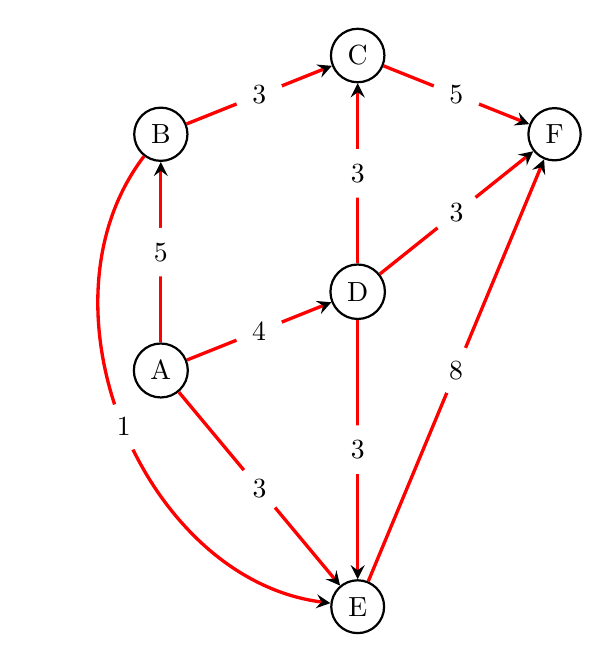
\begin{tikzpicture}
\begin{scope}[every node/.style={circle,thick,draw}]
    \node (A) at (0,0) {A};
    \node (B) at (0,3) {B};
    \node (C) at (2.5,4) {C};
    \node (D) at (2.5,1) {D};
    \node (E) at (2.5,-3) {E};
    \node (F) at (5,3) {F} ;
\end{scope}

\begin{scope}[>={stealth[black]},
              every node/.style={fill=white,circle},
              every edge/.style={draw=red,very thick}]
    \path [->] (A) edge node {$5$} (B);
    \path [->] (B) edge node {$3$} (C);
    \path [->] (A) edge node {$4$} (D);
    \path [->] (D) edge node {$3$} (C);
    \path [->] (A) edge node {$3$} (E);
    \path [->] (D) edge node {$3$} (E);
    \path [->] (D) edge node {$3$} (F);
    \path [->] (C) edge node {$5$} (F);
    \path [->] (E) edge node {$8$} (F); 
    \path [->] (B) edge[bend right=60] node {$1$} (E); 
\end{scope}
\end{tikzpicture}

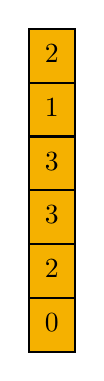
\begin{tikzpicture}[
  thick,
  myrect/.style={
    draw,
    fill=myyellow,
    rectangle split,
    rectangle split parts=#1,
    rectangle split part align=left
    },
  myrect2/.style={
    draw,
    fill=myyellow,
    rectangle split,
    rectangle split draw splits=false,
    rectangle split part align=left
    },  
  mycallout/.style={
    shape=rectangle callout,
    rounded corners,
    fill=mysalmon,
    callout absolute pointer={#1},
    callout pointer width=1cm
  }  
]
\node[myrect=6,text width=1em,align=center]
  (numbers)
  {
  \strut 2
  \nodepart{two}\strut 1
  \nodepart{three}\strut 3
  \nodepart{four}\strut 3
  \nodepart{five}\strut 2
  \nodepart{six}\strut 0
  };
\end{tikzpicture}
\end{comment}
Let's consider a domain decomposition of a numerically solved partial
differential equation (PDE). Let's assume that each processor has $c = O(1)$
terms to communicate between processors. This may be a common case: in a 1D
spatial domain, simple decomposition methods do in fact yield $c = O(1))$ terms
to communicate. Let's say we have a 4-point stencil where value $u^{t+1}_x =
a(u^{t}_{x+1} + u^{t}_{x-1}) + b(u^{t}_{x})$. This produces a backward difference
method in time. When $a = r$ and $b = (1-2r)$ for $r = \kappa / h^2$, this
corresponds to the simplest finite difference approximation for the Heat
equation. When performing this update on a 1D domain, values can be updated for
time $t+1$ independently, except for the dependencies that occur at processor
boundaries. In these cases, the communication of a single value must occur
before updates take place.

Let's assume that we split our domain evenly along the spatial axis. Say we have
a domain such that
\begin{align*}
    x &\in {0, X-1} 
\end{align*}

and that we have $P$ processors in shared memory, and each processor is labeled
\begin{align*}
    p &\in {0, P-1}
\end{align*}

Processor $p$ has a chunk of of the domain with values 
\begin{align*}
    x_p     &= \{\alpha*p, \alpha*(p+1)-1\} \text{, where} \\
    \alpha  &= X / P 
\end{align*}

Given already computed values for $u^{t}_{x} \forall x \in X$, the values for
$u^{t+1}_{x} \forall x \in X$ can be computed in a data parallel manner. But
what dependencies do individual computations at time $t+1$ have on values at
time $t$? The formula provided above makes this quite apparent:
\begin{align*}
    u^{t+1}_{x} \text{ depends on } \{ u^{t}_{x-1}, u^{t}_{x}, u^{t}_{x+1} \}
    \text{.}
\end{align*}

If $x-1$, $x$, and $x+1$ are contained within $x_p$, then these values can be
accessed directly from local memory. $x \in x_p$ by definition. But, if $x =
\alpha*p$ or $x = \alpha*(p+1)$, then communication across processor boundaries
must take place, requiring communication. Communication implies synchronization,
and in order to ensure that the value has been computed, either processor $p-1$
or processor $p+1$ must tell processor $p$ that it has performed that
computation. If processors exist in separate memory spaces, the value must
actually be sent from one memory space to another. Without loss of generality,
let's say processor $p-1$ lags behind in performing its computation
indefinitely. What can processor $p$ do while it waits? It can compute values
for
\begin{align*} 
    u^{t+1}_{x_{t1}} \text{ for } x_{t1} \in \{ \alpha*p + 1, \dots \alpha*(p+1) \} \text{,} \\
    u^{t+2}_{x_{t2}} \text{ for } x_{t2} \in \{ \alpha*p + 2, \dots \alpha*(p+1) \} \text{,} \\
    ... \\
    u^{t+p}_{x_{t\alpha}} \text{ for } x_{t\alpha} \in \emptyset \text{.}
\end{align*}

After $\alpha$ steps through time, processor $p$ must wait for processor $p-1$ to
finish computing its data. Likewise, waiting indefinitely for both processor
$p-1$ and $p+1$ to complete only allows for $\alpha / 2$ steps through time to be
completed. Thus, we can say that
\begin{align*}
    u^{t + i}_{\alpha*p + i-1} \text{ depends on } p-1 \text{, and} \\
    u^{t + i}_{\alpha*(p+1)-1 - (i-1)} \text{ depends on } p+1 \text{, for} \\
    i \in \{ 1, \alpha \} \text{.}
\end{align*}

Each processor has $\alpha$ values to compute per timestep, yielding $\alpha^2$
values to compute in $\alpha$ timesteps. In this range, Processor $p$ has
$\alpha^2/4$ values that do not have dependencies on other processors,
$\alpha^2/2$ values that depend on one adjacent processor, and $p/4$ values that
depend on both adjacent processors. Every time a processor receives a value from
another processor, up to $\alpha$ new values can be computed by $p$ (in the case
that only one adjacent processor's values are needed, and $\alpha/2$ in the case
that both are).

Thus it is in the programmer's best interest to perform communication at points
in time such that each processor always has work to do: either its own work sans
dependencies, or work that relies on values from other processors. Preemptively
aiting for other processors to finish their computation results in more values
it can perform on its own, but of course results in itself being idle. But, only
asking for those values when it absolutely needs them results in a series of
coordination problems... and without the other processor realizing that it
should prioritize communicating the values it depends on, it may have to wait
anyway. Finally, constantly polling to see if adjacent processors have finished
their computation wastes time in itself.

At $t=0$, given an IVP, each processor has the full set of values $u^{0}_{x}
\forall x \in X$. Unsurprisingly, to minimize idle processor time, computing the
values at processor boundaries serves as the best method. Interleaving from
either side, each processor can compute values at spatial points $\alpha*p$,
$\alpha*(p+1) - 1$, $\alpha*p + 1$, $\alpha*(p+1) - 2$, et cetera, for time $t =
1$. At what point in time should it attempt to compute values at time $t = 2$?
If it waits until all values at time $t = 1$ have been computed, it has
performed computations that do not depend on other processors. If later it has
to wait for values its future computations depend on, it has exhausted its own
independent computations on which it could fall back. And, it fails to supply
values that other processors need as early as it can. But, the sooner we try to
compute values at $t = 2$, the more likely that the values we need from adjacent
processors won't have been computed yet.

Stepping back from optimizing execution ordering, consider the following
strategies for dealing with synchronization.

\subsubsection{Preemptive Concurrency Control Scheme}
Commonly, when we synchronize values in shared memory, we perform some check to
see if the value we plan to use has been computed. We may use a spinlock, where
we check if the computing processor has relinquished its lock, and when it has,
we expect the updated value to be in place. Let's call the expected value for
the number of times we must perform this test $\Ev_\text{pre}$. Thus, to
complete a simulation with $T$ timesteps, we incur a runtime overhead of
$O(\Ev_\text{pre} T)$, because we have 2 communications per processor per
timestep; note that $\Ev_{pre}$ may depend on $N$ and $P$ and thus cannot be treated
as a constant.

In a preemptive scheme, $\Ev \geq 1$. Each processor must check to see if its
adjacent processors have computed their values the value preliminarily, and if
the test succeeds, we can use the value straightaway. If the test fails, we may
have to do some unbounded number of checks, say, if processor an adjacent
processor enters an infinite loop.

\subsubsection{Postemptive Concurrency Control Scheme}

In a postemptive scheme, if the adjacent processors to some
processor $p$ have always computed their values before $p$ accesses them, then
there could be potentially no overhead with regard to performing tests. This
precludes any verification of the shared values \-- it does not provide a mechanism
for determining if the values $p$ receives from adjacent processors have, in
fact, derived from the expected computation. This leaves the desire for a scheme
that performs this verification with minimal overhead. Let's call this overhead
$\Ev_\text{post}$.

Consider two processors $p$ and $q$ that are adjacent, and processor $p$
receives value $u^{t}_{x-1}$ from $q$ while computing values for timestep
$t+1$. If values fail to be resolved before multiple
timesteps have taken place on $p$, all three values might need to be resolved.
In the worst case, $p$ completes all of its computation before $q$ has done
anything. Then, $q$ will essentially, by resolving all values in $p$, perform
the entire computation of values in $p$ dependent on $q$ in serial via its
resolution functions. In the best
case, $q$ doesn't have to perform a single resolution, achieving nearly maximal
parallelism. To optimize this process, $p$ should perform computations that are
not dependent on $q$ while $q$ runs its resolution functions; otherwise, it
risks generating more values in need of resolution. Once all resolution has been
performed on a particular value, the reference containing the old version of
that value can be deregistered, which results in it being freed from memory, as
it no longer serves a purpose.

If the resolutions take less time, asymptotically, than the computations
themselves, the algorithm avoids the time wasted by using synchronization
schemes. The difference arises from the fact that as soon as a process computes
a value, it can either operate upon values that that process also has, or values
that another process has. If we limit computation, preemptively, to values local
to a process, the algorithm avoids latency. The algorithm should avoid
communication until absolutely necessary.

\begin{comment}
Let's assume that we split our domain evenly along both spatial axis. Say we
have a domain such that
\begin{align*}
    i &\in {0, M-1} \\
    j &\in {0, N-1}
\end{align*}

and that we have $P$ processors in shared memory, and each processor is labeled
\begin{align*}
    p &\in {0, P-1}
\end{align*}

Processor $p$ has a chunk of of the domain with values 
\begin{align*}
    i_p     &\in {\alpha*p, \alpha*(p+1)} \times {\beta*p, \beta*(p+1)} \text{, where} \\
    \alpha  &= M/\log{P} \% \log{P} \text{ and} \\
    \beta   &= N/\log{P} /  \log{P} \text{.}
\end{align*}

\begin{verbatim}
compute in shared memory all values for p_r
determine set of values to share: could be 1...s rows
serialize; mpi_isend start
mpi_irecv start; deserialize (should be free)
for each node that uses ghost node data:
compute f(data_local, data_sent)
\end{verbatim}
\end{comment}

 % Methods

\lhead{\emph{Implementation}}
\chapter{Implementation}

\section{Overview of Interface}
The fundamental structure that affords parallelism without data races is the
bit-partitioned P/T vector. This vector can be created and used like a C++
standard library vector (with some limitations) and can be modified at will in
parallel environments. If used in this way, each process will continuously
generate new, immutable versions of the persistent vector with each operation it
performs, and thus each process will have its own view of the vector,
independent of the others. Any given process cannot see the operations performed
by the other processes. So, this affords us consistency with respect to reading
the contents of these vectors, but not with writing.

\subsection{Splinters, Detaching, and Reattaching} In order to get consistency
with respect to writing, the concepts of \texttt{detach} and \texttt{reattach}
come into play. A P/T vector can be \textit{detached} off another P/T vector,
operated upon, and later \textit{reattached} onto an output vector. These
operations take place in a single process, and the \textit{splinter} that was
detached allows for non-blocking, asynchronous, parallel operations. The series
of vectors slated for detaching and reattaching determines the global ordering
of the operations. A \texttt{detach} that comes before a \texttt{reattach} sees
the data structure as it was before the corresponding operations that conclude
via that join. A \texttt{detach} that comes after a \texttt{reattach} sees the
data structure as it was after the corresponding operations that conclude via
that join. Orderings where there are two paired detaches and reattaches where
both \texttt{detach} calls come before both \texttt{reattach} calls imply that
the two operations are commutative and associative with each other, and the
ordering doesn't matter. Both operations see each other, and the final result
will be consistent if the commutativity and associativity of those operations
hold. If they do not, different results will arise from different arbitrary
orderings of those two operations with respect to each other; this is
semantically correct behavior and could very well be intentional.  Here the
semantics state that the logical ordering of the two operations is simultaneous,
that they occur at the same point in time relative to a global logical clock.

\subsection{Limitations of Splinters}
When a user operates upon a splinter, it can only do so via methods
available for that vector. It cannot arbitrarily write values into locations of
the vector; while there are ways to address add and remove operations on P/T
vectors, for now we will focus on vectors whose size do not change.
These methods allow pre-specified operations to be performed on some subset of
values in the vector. The user can create these operations by instantiating
instances of an \texttt{operator} and then tag the instances as being associative and/or
commutative. In addition, pairs and sets of operators can have operations
defined relative to each other, so that if multiple operators are used among
different splinters with the same parent (a P/T vector), that resolution can
be optimized to allow the most lenient orderings that do not invalidate the
result. Each splinter has a fixed operator it uses for its lifetime. 
This \texttt{compute} method takes a value to use with that operator and an index that 
determines the value in the splinter upon which the operator will be applied.

\subsection{Resolving}
Finally, there is a \texttt{resolve} method that forces blocking, synchronous
resolution from one P/T vector onto another, its \textit{dependent}. 
This allows the user to perform intermittent i/o
with consistent results, and for the user to create an ending terminus for a
computation subgraph that supports resolution. If values from a P/T vector are
to be used in a non-P/T context, the values must be fully resolved in order to
to obtain consistent results from that point forward.

So, if the inputs to \texttt{compute} for use with the passed operator are values in 
P/T vectors, then the resulting vector will be treated as a \textit{dependent} of those 
vectors. Otherwise, the P/T vector that performs
the \texttt{compute} will be treated as the starting terminus of any resolutions in its 
computation subgraph.

\subsection{Aggregate Operations}
The library also contains a \texttt{stencil} function that takes an operator,
another P/T vector, and a set of relative indices; it then performs a 
\textit{stencil} operation, where it uses the values at those indices relative to
any/every index for the passed P/T vector as the arguments for the operator
provided, placing the results in a new P/T vector returned and ignoring
out-of-bounds indices. The function still takes iterators into the input vector
to determine the range that the stencil is applied. (Note that this equates to
performing a diagonal matrix/vector multiplication in the case where the iterators
delineate the entire input vector. See the Future Directions section below for a
detailed plan moving forward for a full specification of a linear algebra
library that could develop from this much simpler function.) This also allows
the resulting vector to receive updates if and when resolutions take place on
the dependent vectors used to produce it. Dependencies on singular values can be
encoded by passing a relative index vector of size 1 and iterators that only
select one value in the vector, and in this case a vector of size 1 is returned.
Likewise, a proxy for a reduce operation involves an index vector indicating
every other value in the array and iterators that only select one value in the
vector.

There are two other aggregate functions, \texttt{foreach} and \texttt{reduce}, that are
special cases of \texttt{stencil}. The
former takes two iterators (instead of a single index) that determine the start
and end points in the vector where the operator will be applied and either a value to use 
with the operator on that range, or another P/T vector whose values will be used along 
that range. The latter takes two iterators, and reduces the values in the calling 
vector onto the 0-index spot of a returned vector that has size 1.

\subsection{Partitioning and Indexmaps}
When an aggregate function is called on a P/T vector, the appropriate \texttt{compute} 
operations are slated for execution, and each available process receives a partitioned 
portion of the task. The details for the \texttt{foreach} and \texttt{reduce} functions 
are described below. The details are given here because they generalize to operations 
that are data-parallel with an identity \textit{index mapping} or \texttt{indexmap}, and with an 
all-to-one \texttt{indexmap}, respectively. Any other aggregate function boils down into some 
combination of these forms of data-parallelism. In general, the \texttt{indexmap} has a domain 
and a range. The domain consists of addresses of values that comprise those used for 
the aggregate function, and the range consists of addresses of values in the resulting, 
dependent P/T vector. The \texttt{indexmap} itself relates which input addresses 
go into the production of a given output address. When a separate \texttt{indexmap} is 
provided for each input which is also a P/T vector, the addresses simply become integral 
indices into those vectors. In these special cases, the internal structure of the P/T 
vector as nodes with either $k$ branches (internal nodes) or $k$ values (leaves). This 
structure allows us to minimize the amount of work necessary to partition the individual 
\texttt{compute} operations in a data-parallel way that avoids conflicts (and thus 
possibly costly resolutions) down the line. But, in general, it is possible to identify 
and minimize the number of potential conflicts which must be tested for detection and 
subsequent resolutions which must be then performed for all detected conflicts.

The \texttt{foreach} function is split among processes in a data parallel
manner. The P/T vector is split into $k^d$ nodes at each depth $d$  of the
underlying trie. If there are $P$ processes and $n$ values in the vector with
depth $d = \ceil{\log{n}}$, The tree is ascended to depth $d'$ where $k^{d'} \geq P$
but ${k-1}^{d'} < P$, and each internal node $i \in \{0, \dots k^{d'}\}$ are
partitioned in chunks of $k$ with the final process receiving a smaller chunk if
necessary. Using an iterator, each process can move to the first value in the
vector it owns and performs the operation at up to $k$ nodes forward at that
depth, stopping if it reaches the end of the vector.

The \texttt{reduce} function is split into a $P$ chunks of values to be reduced.
Each process reduces its chunk of values in serial, and then one processor
reduces the resulting $P$ values. If $P > k$, the values will be
reduced in chunks of $k$ until there are just $k$ values left, and then one
process $P$ will reduce those resulting $k$ values, finally writing the final
value as the output, or to the resulting place in another $P/T$ vector, tagged
with the operation given for the reduction. if $P \leq k$, a single process will
reduce the values.

This constitutes a fairly simple strategy for scheduling work in a balanced
manner among processes. Alternative and potentially more robust solutions are
discussed in the following Future Directions section.

\section{Dependency Tracking, Conflict Detection, and Resolution}
When a detach/reattach group begins, the first course of action is to create
the output P/T vector and label it as being dependent on the calling vector.
When this happens, some other bookkeeping takes place to in order to manage the
ensuing contention of data among parallel processes.

\subsection{Freezing}
When P/T vectors are used as inputs for operations, they must be \textit{frozen}
prior to those operations taking place. To \texttt{freeze} a vector, one must supply the
complete set of dependee P/T vectors and have created the dependent vector where the
operation's result will exist, in addition to the operators and index mappings
that relate those dependents to the resulting vector. Each operation has a
primary input and auxiliary inputs. The primary input is the vector that the
user thinks of operating upon, and the auxiliary inputs can be seen as helpers,
such as a list of coefficients by which to multiply each value in an input
vector, for example.

\subsection{Tracking}
The registration process stores the \texttt{operator} and \texttt{indexmap} in a struct
called a \textit{tracker}. It also stores a snapshot of the input vector, which it
will use to perform its computations. It needs this because in order to
correctly perform conflict detection and resolution, it must have a persistent,
immutable reference to the input at the time it was used. Otherwise, subsequent
updates to the input may render the reference inconsistent between its use and
the conflict/detection and resolution processes. The tracker obtains the
snapshot by atomically copy-constructing the P/T vector into the tracker (which
only really does a \texttt{shared\_ptr} copy of the root node of the P/T vector)
and giving the input P/T vector a new id. Now that the input has a new id, any
value that it updates will construct new nodes throughout the entire path to the
modified value, and the copy in the tracker will remain untouched. This snapshot
of the input can thus be seen as frozen at the point in time that this
preparation takes place.

\subsection{Reattach Latches}
Finally, the freezing process also creates a \textit{latch} with a count for each
splinter that will work on this compute. This count has a default that can be
set at compile-time. When the splinters are finished, they reattach their
computed values to the output vector and decrement the count. When the count
reaches 0, the computation is complete, save for resolution that may or may not
need to take place. The Boost C++ library provides an implementation of a latch with 
this precise interface.

\subsection{Differences in the Treatment of Primary and Auxiliary Input}
The final step of latch creation happens for the primary input as expected, but for 
auxiliary inputs, it uses a value of 0 to avoid redundancy. 
Instead, the freezing process for non-primary inputs takes the primary input as an 
argument as well, and adds it to a list of auxiliary frozen inputs for that particular
computation. When resolution happens from the primary input onto the output, it resolves 
the auxiliary inputs as well, once it has finished performing its own resolution. In 
this way it will always only resolve once the relevant splinters have reattached, and 
the user will only have to call resolve once per computation.

\subsection{Detach and Reattach, in Context}
The user then calls a method called \texttt{detach} from any of the threads it created 
to perform asynchronous, parallel computation. It is returned with a splinter that it 
can operate on using the single-index \texttt{compute} method described above. If the 
user intended to operate upon the input during this computation, the  
splinters have the same contents as the frozen snapshot of the input, which is achieved 
by copying the snapshot and incrementing the id of the splinter's copy; now, splinters 
will have to construct new nodes to the modified value as well, but only for the values 
that they modify. The user 
must either be careful to compute either with non-P/T values, or to compute with values 
in a P/T vector it specifically froze for the task, using the relevant \texttt{indexmap}, and in 
both cases, the relevant operator (though, the correct operator will be used via the
\texttt{compute} method of the splinters). Failing to do so will result in an inconsistent 
resolution process, whether or not that leads to inconsistent values themselves.

Once the user is done, they call \texttt{reattach} to connect each splinter to the output 
vector. The \texttt{reattach} method will do its best to efficiently assign the values 
of the output vector as necessary. If the splinters performed data-parallel operations 
with index mappings that have contiguous output values of groups of at least the branch size 
of the P/T nodes, then \texttt{reattach} will be able to leverage the internal trie 
structure of P/T vectors such that this operation takes place in as little as $\mathcal{O}(1)$
time.

Detaching and reattaching must be paired for each splinter, sandwiched by calls to
\texttt{compute}, and exactly $P_s$ calls to both must take 
place, where $P_s$ is the number of splinters specified when freezing. Within 
\texttt{reattach}, the latch is decremented; if the latch decrements below 0, the code 
will terminate.

\subsection{Resolution}
At any point, the user may choose to never resolve the P/T vectors if desired. If the 
user decides that they do not actually care to see the finalized values in those 
vectors, they may choose to leave them unresolved, incurring no runtime penalty for 
synchronization. Otherwise, the user must resolve P/T vectors in the order that they 
were computed upon; resolving P/T vectors that used another P/T vector as a dependent 
without first resolving the dependent will not work, because the vector which performs 
the resolution onto the dependee must, logically, be finalized in order for resolution 
to take place. During resolution, the finalized input vector compares its values to the 
frozen version of it that the splinters used. If the values differ, it uses the inverse
of the operator to determine what the relevant difference is, and the operator itself to
update the value in the output vector. This, of course, relies on the invertibility of 
the operator. Non-invertible operators cannot be used with P/T vectors.

If the resolution process required looking at every value in the output vector, this 
process would take too prohibitively long to yield a useful method. But, the \texttt{indexmap} 
provided for the computation gives the process information about which values are prone 
to conflicts. If the user partitions the addresses that the splinters modify (the range of 
the \texttt{indexmap}), then the only  values that may need resolution are ones for 
whom within a given splinter's range of the \texttt{indexmap}, value(s) in their domain 
lie(s) outside that range. This is so because within splinters, 
operations on P/T vectors happen sequentially, so splinters always see finalized values 
at indices that lie within their range of the \texttt{indexmap}. It can be seen that for 
purely data-parallel operations (such as \texttt{foreach} operations), there are no 
dependents, and that, say, for a stencil that uses adjacent values in the P/T vector, 
only $2(P-1)$ values must be checked, at each internal boundary between 
the splinters. If index mappings are provided in code as \texttt{constexpr} functions and the number 
of splinters is provided in code as a \texttt{const} value, a partition of the range and the 
corresponding indices with possible conflicts can be determined at compile-time.
Furthermore, it is possible to was that really it???????? GOOD JOB SEAN!!!
 % Implementation

\lhead{\emph{Results}}
\chapter{Results}

Results are shown from two machines.

The first machine has a dual-core Intel IvyBridge i7-3520M processor with 12GB
RAM running Debian Jessie/Stretch using g++ 6.1.1.

The second machine has 2 quad-core AMD Opteron 4386 processors with 64GB RAM
running Ubuntu 14.04 LTS using g++ 5.4.0.

Tests are performed on each machine up to twice the number of physical threads;
the maximum number of threads tested are thus 4 and 16. These utilize hyperthreading
to run two simultaneous threads per core, but hyperthreads will not necessarily
provide the same performance as running each thread on its own physical core [cite].



\section{Reduce}
Results shown compare various implementations of a reduce operation of a random
vector of doubles:

\begin{itemize}
 \item ``seq'' is a sequential implementaiton;
 \item ``vec'' is a sequential implementation, but with values always stored in
 vectors (e.g., results of ``reduce'' operations are stored in size-1 vectors).
 This is provided because in order for this method to operate in parallel on
 vectors, the result operations must be itself stored in a ctvector, for
 comparison's sake, tests are performed with the same restriction with a
 std::vector;
 \item ``omp'' is an OpenMP implementation. It uses the maximum number of cores
 available in all cases, so it is also not sensitive to the number of
 threads/cores that are manually selected;
 \item ``avx'' uses a 256-bit AVX instruction to perform the addition of 4 doubles
 simultaneously until only 4 values remain, and then uses more avx instructions
 to sum the resulting values. Thus, the speedup of this implementation can be
 compared directly to other implementations when using 4 concurrent threads;
 \item ``async`` is a C++11-style parallel implementation using the C++ std::async
 feature to launch threads, each of which are given a fraction of the list equal
 to the inverse of the total number of threads.
\end{itemize}

\begin{figure}[!h]
\centering
    \includegraphics[width=0.5\textwidth]{Graphs/boostfunc/reduce_size-v-time.png}
\end{figure}
\begin{figure}[!h]
\centering
    \includegraphics[width=0.5\textwidth]{Graphs/boostfunc/reduce_procs-v-speed-s.png}
\end{figure}
\begin{figure}[!h]
\centering
    \includegraphics[width=0.5\textwidth]{Graphs/boostfunc/reduce_procs-v-speed-m.png}
\end{figure}
\begin{figure}[!h]
\centering
    \includegraphics[width=0.5\textwidth]{Graphs/boostfunc/reduce_procs-v-speed-l.png}
\end{figure}

\section{Foreach}
Results show strong and weak scaling for the contentious library performing a
foreach operation on a random vector of doubles. For comparison, the results
show the runtime of a serial implementation as well.

\section{Heat}
Results show strong and weak scaling for the contentious library using a
1st-order scheme to compute the heat equation framed as a Boundary-Value
Problem.

\begin{comment}
With optimization turned on vec behaves a lot like seq. Without
optimization, vec is a lot slower. All these benchmarks use optimization flags,
so the results are almost identical between seq and veche "async"
implementation uses C++ threads with the async
\end{comment}
 % Results and Discussion

\lhead{\emph{Conclusion}}
\chapter{Discussion}

Postemptive concurrency control strategies naturally flourish in settings with
low contention and aid the programmer especially when that contention doesn't
always have a predetermined structure. As demonstrated, such strategies allow
for levels of parallelism comparable to current methods and adapt well to the
fact that different parallel runs incidentally produce different degrees of
parallelism. But, the lack of explicit contention management serves as perhaps
the most attractive aspect of postemptive strategies. When using preemptive
strategies, the correctness of the program depends on the ability of the
programmer to explicitly manage concurrent reads and writes of shared data.
Historically it has proven a time-consuming and complex task. Postemptive
concurrency control schemes avoid the need for this and allow for reads and
writes to shared data under common and practical use cases. Their downsides
involve potential decreases in the runtime and space efficiency of the program
and the need to supply extra information about the behavior of the program. But,
in practical settings, it remains to be seen whether postemptive methods such as
the one described competes with optimized preemptive methods.

\section{Optimization of Implementation}
There are a number of existing optimizations to CT vectors that are not present
in the current implementation.

\subsection{Memory Allocation of Nodes and Leaves}
One major source of slowdown in the \texttt{ctvector} implementation of the
tests comes from freeing and allocating nodes needed by the vector whenever a
thread  modifies a leaf of a splinter it has not yet modified since detaching.
Many programs involve repeatedly detaching/reattaching as part of an iterative
process, meaning that nodes and leaves will freed and allocated at a similar
pace; furthermore, every node will have the same size as every other node, and
likewise for leaves. A custom allocator could avoid unnecessary allocations by
reusing freed leaves when allocating new ones, which would reduce the overall
time spent allocating and freeing memory.

\begin{comment}
TODO: move to implementation
\subsection{Redundant Storage in Nodes}
The size of the code could be reduced by a fairly
large constant factor of approximately $2$ for 32-bit values (such as
\texttt{int}s or \texttt{float}s on most platforms) and a depth of $5$, which
corresponds to a size of $64^5 \approx 1,000,000,000$ using the default branch
size of 64. This factor diminishes to $1.07$ for storing 1024-bit objects and
increases to $3.4$ for packed boolean values by using a \texttt{std::bitset}
instead of a \texttt{std::array} to store values, although this has not been
implemented. In space-sensitive applications where computations are usually
performed on 32-bit numbers, the space savings above do make a difference.
\end{comment}

\subsection{Tail Optimization}
The CT vector can benefit from a tail optimization where the pointer to
the final leaf is stored in the root. This optimization primarily benefits
inserting at the end of the tree, and since the CT vector was primarily
leveraged for mutations as opposed to inserting and removing elements, this
optimization was not prioritized.

\subsection{Branching Factor}
The CT vector's nodes stores a constant number of branches or values where that
constant is some power of 2, in order to provide an efficient method for lookup
of values through the tree. When the constant is 32 or greater, the runtime of
traveling to a leaf is at most $\log_{32}(n)$ where $n$ is the size of the
vector. It is unfeasible to store more than 256 billion bytes in memory (this
corresponds to a processor that has access to 256 gigabytes of shared memory),
and it is unrealistic to store objects smaller than one byte.
$\log_{32}(256,000,000,000) \approx 7.58$, which means that the depth of the
bit-partitioned trie of nodes and leaves will never exceed 8. With a branching
factor of 64 and a vector with at most 1 billion values, the depth will never
exceed 5. This growth is so slow that it can, for all intents and purposes, be
treated as a constant, which is why a large branching factor is used. But, the
larger the branching factor, the larger the copy when a CT vector sets a value
in a node it has not yet touched, as it must copy entire nodes. Picking a
contextually good branching factor, or even dynamically determining it or using
heterogeneous branching factors for different parts of the trie, could improve
performance.

In the setting of automated parallelism, often the pattern by which splinters
will access and mutate the input vector is known in advance. When this is the
case, it may be possible to choose a branching factor for points in the vector
that corresponds to those access and mutation patterns. It is much more
efficient for splinters to mutate whole leaves, or better yet, whole subtries,
and the shallower the root of the subtrie in the CT vector, the more efficient
the process. Tailoring the branching structure of the trie to confer these ideal
conditions would result in an optimal reattaching and resolution process.
Furthermore, assuming a sparse access and mutation pattern, the trie could even
change its branching factor at runtime to minimize copying and to avoid
unnecessary checking during reattachment and resolution, by keeping the size of
newly-created leaves as small as possible. It remains to be seen whether the extra
logic necessary to manage a bit-partitioned trie with nodes that do not always
have the same branching factor would outweigh the optimizations made possible by
that flexibility, or vice-versa.

\subsection{Computation Ordering to Minimize Contention}
When the range of the indexmap is partitioned among splinters, the domain does
not necessarily partition in the same way. Any values in the domain that lie
outside a given splinter's range are candidates for conflicts. These are the
values checked in the resolution process. By having splinters compute these
values first, the chance that conflicts will occur is minimized.
This optimization has not been implemented, and it remains to be seen if the
extra logic necessary to compute the values in a non-consecutive order can be
implemented without the overhead outweighing the benefits. Furthermore,
performing operations on non-contiguous data can cause cache misses, and so the
unpreditable behavior of hardware might limit the performance of this strategy.
It is likely that there are cases, such as multi-dimensional finite difference
stencils, where the sparsity and pattern of values with potential conflicts are
straightfoward enough to easily prioritize the slated operations.

\subsection{Optimization of operators and indexmaps}
Operators and indexmaps are currently stored in structs with
\texttt{std::function} objects inside them. While this provides an elegant
interface for dealing with functions logically in C++, this standard library
function type does not allow for the same level of optimization as raw C-style
function pointers, or better yet, truly inline operations that map to an
optimized set of assembly instructions. For operations with relatively few (or
even exactly 1) assembly instructions, the overhead of working with
\texttt{std::function} objects adds too much overhead to the execution of the
functions contained within. The inability of the C++ compiler to inline
functions stored as these types exacts the majority of the overhead. A more
efficient interface for managing functions as variables and working with them
symbolically is necessary for this vector to be truly competitive with standard
implementations. Likely this will involve some combination of C-style function
pointers and templated functions that have template parameters that receive
those function pointers.

\subsection{Fully lock-free Reattaching and Resolution}
Currently the CT vector implementation uses two locks: one to lock the map where
trackers are stored when they are emplaced into the map, and another to lock the
dependent vector's bit-partitioned trie when reattaching of reduce-style
partitions and when resolution happens. The first lock is necessary and does not
affect performance, because the emplacement of values into this map and lookups
in the map accounts for very little actual work compared to the amount of work
splinters would do in actual uses cases for parallelisim. The second lock has
two uses. In the first, really a single processor should perfrom this
reattachment, because each processor holding a lock to perform the final reduce
of $P$ or fewer values incurs substantial overhead compared to a simple serial
reduce. In the second, locking prevents the need to resolve again with the same
dependee-dependent pair after resolution takes place if an output vector depends
on multiple input vectors.  The code has not yet been configured to rerun
resolution in the correct sequence to avoid this lock, although as described it
is possible to achieve resolution in a totally lock-free manner.

The only other synchronization primitive used is a
\texttt{std::atomic<int32\_t>} for assigning IDs to CT vectors (and raw
transient vectors, if used).

\section{Improvement of Interface}

\subsection{The Copying Problem}
CT vectors do not have consistent semantics for being copied by value. Currently
when the user calls the copy constructor on a CT vector, it returns a copy of
the underlying bit-partitioned vector with a new ID and an otherwise empty set
of members. Passing a CT vector by value to a method and expecting it to behave
like a genuine copy of the original vector does not work. It will not be able to
serve as a candidate for detaching or reattaching splinters as if it were the
original vector, and additionally will not be able to serve as a base for
resolution of vectors that were produced by using the original vector as input.
This is, of course, the correct behavior, but accidentally calling the copy
constructor in various situations may confuse users.

Developing a better interface and writing a semantically correct move
constructor would solve this problem.

\subsection{The Intermediate Dependencies Problem}
One major concern involves
writing subroutines that perform multiple stepwise computations (where each step
involves a set of splinter detach and reattach calls) from a local function
scope, where the function returns the final output vector. In order to preserve
the asynchronous properties of the CT vector, the intermediate functions must
be resolved outside the local function scope, or else the resolution will be
premature and force synchronization when the function returns. But, there is no
good way of moving those intermediate CT vectors outside of the local function.
Currently, the destructor of the CT vector waits for all detached splinters to
reattach, as otherwise, segfaults will take place while the splinters do try to
reattach. The destructor does not perform forward resolution or wait for itself
to be resolved; doing so would prevent the desired asynchronous properties.
Resolving onto a vector that has been destroyed (by being \texttt{delete}d if
allocated on the heap, or by going out of scope) is currently undefined behavior
in the same way that using any deleted object is undefined behavior. This is why
the interface requires that the vectors being resolved onto are passed manually
as parameters: it forces users to have undeleted and in-scope references to
them in order to perform resolution on them.
 % Conclusion
%Term definitions
\glsaddall
%% ----------------------------------------------------------------
% Now begin the Appendices, including them as separate files

\addtocontents{toc}{\vspace{2em}} % Add a gap in the Contents, for aesthetics
%
\appendix % Cue to tell LaTeX that the following 'chapters' are Appendices
%
\chapter{Additional Benchmark Results}

Results from running the benchmarks described in the results section using a
dual-core Intel IvyBridge i7-3520M processor with 12GB RAM running Debian
Jessie/Stretch using g++ 6.1.1.

\begin{figure}[!h]
\centering
    \includegraphics[width=0.76\textwidth]{Figures/reduce+foreach/reduce_size-v-time.png}
\end{figure}
\begin{figure}[!h]
\centering
    \includegraphics[width=0.76\textwidth]{Figures/reduce+foreach/reduce_procs-v-speed-s.png}
\end{figure}
\begin{figure}[!h]
\centering
    \includegraphics[width=0.76\textwidth]{Figures/reduce+foreach/reduce_procs-v-speed-m.png}
\end{figure}
\begin{figure}[!h]
\centering
    \includegraphics[width=0.76\textwidth]{Figures/reduce+foreach/reduce_procs-v-speed-l.png}
\end{figure}
\begin{figure}[!h]
\centering
    \includegraphics[width=0.76\textwidth]{Figures/reduce+foreach/reduce_procs-v-speed-a.png}
\end{figure}

\begin{figure}[!h]
\centering
    \includegraphics[width=0.76\textwidth]{Figures/reduce+foreach/foreach_size-v-time.png}
\end{figure}
\begin{figure}[!h]
\centering
    \includegraphics[width=0.76\textwidth]{Figures/reduce+foreach/foreach_procs-v-speed-a.png}
\end{figure}

\begin{figure}[!h]
\centering
    \includegraphics[width=0.76\textwidth]{Figures/heat/heat_size-v-time.png}
\end{figure}
\begin{figure}[!h]
\centering
    \includegraphics[width=0.76\textwidth]{Figures/heat/heat_width-v-speed-a.png}
\end{figure}
\begin{figure}[!h]
\centering
    \includegraphics[width=0.76\textwidth]{Figures/heat/heat_steps-v-speed-a.png}
\end{figure}

	% Appendix Title

%\input{Appendices/AppendixB} % Appendix Title

%\input{Appendices/AppendixC} % Appendix Title
\addtocontents{toc}{\vspace{2em}}  % Add a gap in the Contents, for aesthetics
\backmatter

%% ----------------------------------------------------------------
%\label{Glossary}
%\lhead{\emph{Glossary}}
%\printglossaries

\label{Bibliography}
\lhead{\emph{Bibliography}}  % Change the left side page header to "Bibliography"
\printbibliography  % The references (bibliography) information are stored in the file named "Bibliography.bib"

\end{document}  % The End
%% ----------------------------------------------------------------
